\documentclass[twoside]{book}

% Packages required by doxygen
\usepackage{fixltx2e}
\usepackage{calc}
\usepackage{doxygen}
\usepackage[export]{adjustbox} % also loads graphicx
\usepackage{graphicx}
\usepackage[utf8]{inputenc}
\usepackage{makeidx}
\usepackage{multicol}
\usepackage{multirow}
\PassOptionsToPackage{warn}{textcomp}
\usepackage{textcomp}
\usepackage[nointegrals]{wasysym}
\usepackage[table]{xcolor}

% Font selection
\usepackage[T1]{fontenc}
\usepackage[scaled=.90]{helvet}
\usepackage{courier}
\usepackage{amssymb}
\usepackage{sectsty}
\renewcommand{\familydefault}{\sfdefault}
\allsectionsfont{%
  \fontseries{bc}\selectfont%
  \color{darkgray}%
}
\renewcommand{\DoxyLabelFont}{%
  \fontseries{bc}\selectfont%
  \color{darkgray}%
}
\newcommand{\+}{\discretionary{\mbox{\scriptsize$\hookleftarrow$}}{}{}}

% Page & text layout
\usepackage{geometry}
\geometry{%
  a4paper,%
  top=2.5cm,%
  bottom=2.5cm,%
  left=2.5cm,%
  right=2.5cm%
}
\tolerance=750
\hfuzz=15pt
\hbadness=750
\setlength{\emergencystretch}{15pt}
\setlength{\parindent}{0cm}
\setlength{\parskip}{3ex plus 2ex minus 2ex}
\makeatletter
\renewcommand{\paragraph}{%
  \@startsection{paragraph}{4}{0ex}{-1.0ex}{1.0ex}{%
    \normalfont\normalsize\bfseries\SS@parafont%
  }%
}
\renewcommand{\subparagraph}{%
  \@startsection{subparagraph}{5}{0ex}{-1.0ex}{1.0ex}{%
    \normalfont\normalsize\bfseries\SS@subparafont%
  }%
}
\makeatother

% Headers & footers
\usepackage{fancyhdr}
\pagestyle{fancyplain}
\fancyhead[LE]{\fancyplain{}{\bfseries\thepage}}
\fancyhead[CE]{\fancyplain{}{}}
\fancyhead[RE]{\fancyplain{}{\bfseries\leftmark}}
\fancyhead[LO]{\fancyplain{}{\bfseries\rightmark}}
\fancyhead[CO]{\fancyplain{}{}}
\fancyhead[RO]{\fancyplain{}{\bfseries\thepage}}
\fancyfoot[LE]{\fancyplain{}{}}
\fancyfoot[CE]{\fancyplain{}{}}
\fancyfoot[RE]{\fancyplain{}{\bfseries\scriptsize Generated by Doxygen }}
\fancyfoot[LO]{\fancyplain{}{\bfseries\scriptsize Generated by Doxygen }}
\fancyfoot[CO]{\fancyplain{}{}}
\fancyfoot[RO]{\fancyplain{}{}}
\renewcommand{\footrulewidth}{0.4pt}
\renewcommand{\chaptermark}[1]{%
  \markboth{#1}{}%
}
\renewcommand{\sectionmark}[1]{%
  \markright{\thesection\ #1}%
}

% Indices & bibliography
\usepackage{natbib}
\usepackage[titles]{tocloft}
\setcounter{tocdepth}{3}
\setcounter{secnumdepth}{5}
\makeindex

% Hyperlinks (required, but should be loaded last)
\usepackage{ifpdf}
\ifpdf
  \usepackage[pdftex,pagebackref=true]{hyperref}
\else
  \usepackage[ps2pdf,pagebackref=true]{hyperref}
\fi
\hypersetup{%
  colorlinks=true,%
  linkcolor=blue,%
  citecolor=blue,%
  unicode%
}

% Custom commands
\newcommand{\clearemptydoublepage}{%
  \newpage{\pagestyle{empty}\cleardoublepage}%
}

\usepackage{caption}
\captionsetup{labelsep=space,justification=centering,font={bf},singlelinecheck=off,skip=4pt,position=top}

%===== C O N T E N T S =====

\begin{document}

% Titlepage & ToC
\hypersetup{pageanchor=false,
             bookmarksnumbered=true,
             pdfencoding=unicode
            }
\pagenumbering{roman}
\begin{titlepage}
\vspace*{7cm}
\begin{center}%
{\Large b-\/car }\\
\vspace*{1cm}
{\large Generated by Doxygen 1.8.11}\\
\end{center}
\end{titlepage}
\clearemptydoublepage
\tableofcontents
\clearemptydoublepage
\pagenumbering{arabic}
\hypersetup{pageanchor=true}

%--- Begin generated contents ---
\chapter{Todo List}
\label{todo}
\hypertarget{todo}{}

\begin{DoxyRefList}
\item[\label{todo__todo000002}%
\hypertarget{todo__todo000002}{}%
Global \hyperlink{group__car_ga6b1fd674445dd1c654dfe8b8b65f168e}{beam} (unsigned long state)]Rewrite as all L\+E\+Ds get clear at the begining of the main loop  
\item[\label{todo__todo000001}%
\hypertarget{todo__todo000001}{}%
File \hyperlink{car__basics_8ino}{car\+\_\+basics.ino} ]Write a function for brake lights.  
\item[\label{todo__todo000003}%
\hypertarget{todo__todo000003}{}%
File \hyperlink{police_8ino}{police.ino} ]May add more flasher. 

Extract beacon light as seperate function.  
\item[\label{todo__todo000004}%
\hypertarget{todo__todo000004}{}%
File \hyperlink{rainbow_8ino}{rainbow.ino} ]Make period of rainbow cycle configurable in \hyperlink{config_8h}{config.\+h}  
\item[\label{todo__todo000005}%
\hypertarget{todo__todo000005}{}%
File \hyperlink{speed_8ino}{speed.ino} ]Write a function that detects braking via negaive acceleration. 
\end{DoxyRefList}
\chapter{Module Index}
\section{Modules}
Here is a list of all modules\+:\begin{DoxyCompactList}
\item \contentsline{section}{Buttons}{\pageref{group__buttons}}{}
\item \contentsline{section}{Car Basics}{\pageref{group__car}}{}
\item \contentsline{section}{Knight Rider}{\pageref{group__knightrider}}{}
\item \contentsline{section}{Police}{\pageref{group__police}}{}
\item \contentsline{section}{Rainbow}{\pageref{group__rainbow}}{}
\item \contentsline{section}{Speed}{\pageref{group__speed}}{}
\item \contentsline{section}{Deployment}{\pageref{group__deployment}}{}
\item \contentsline{section}{Main}{\pageref{group__main}}{}
\item \contentsline{section}{Fast\+L\+ED}{\pageref{group___fast_l_e_d}}{}
\item \contentsline{section}{Adafruit\+\_\+\+Neo\+Pixel examples}{\pageref{group___adafruit}}{}
\end{DoxyCompactList}

\chapter{File Index}
\section{File List}
Here is a list of all files with brief descriptions\+:\begin{DoxyCompactList}
\item\contentsline{section}{\hyperlink{b-car_8ino}{b-\/car.\+ino} \\*Main file }{\pageref{b-car_8ino}}{}
\item\contentsline{section}{\hyperlink{buttons_8ino}{buttons.\+ino} \\*Use two R-\/2R resistor ladder networks to connect up to 10 buttons on two analog inputs }{\pageref{buttons_8ino}}{}
\item\contentsline{section}{\hyperlink{car__basics_8ino}{car\+\_\+basics.\+ino} \\*Basic car functionality }{\pageref{car__basics_8ino}}{}
\item\contentsline{section}{\hyperlink{config_8h}{config.\+h} \\*Adjust your settings here }{\pageref{config_8h}}{}
\item\contentsline{section}{\hyperlink{knightrider_8ino}{knightrider.\+ino} \\*Knight Rider like front row }{\pageref{knightrider_8ino}}{}
\item\contentsline{section}{\hyperlink{police_8ino}{police.\+ino} \\*Police beacon light and front flash }{\pageref{police_8ino}}{}
\item\contentsline{section}{\hyperlink{rainbow_8ino}{rainbow.\+ino} \\*Rainbow effect functions }{\pageref{rainbow_8ino}}{}
\item\contentsline{section}{\hyperlink{speed_8ino}{speed.\+ino} \\*Measure speed }{\pageref{speed_8ino}}{}
\item\contentsline{section}{\hyperlink{utils_8ino}{utils.\+ino} \\*Collection of utils }{\pageref{utils_8ino}}{}
\end{DoxyCompactList}

\chapter{Module Documentation}
\hypertarget{group__buttons}{}\section{Buttons}
\label{group__buttons}\index{Buttons@{Buttons}}


Use R-\/2R resistor ladder network for more buttons.  


\subsection*{Files}
\begin{DoxyCompactItemize}
\item 
file \hyperlink{buttons_8ino}{buttons.\+ino}
\begin{DoxyCompactList}\small\item\em Use two R-\/2R resistor ladder networks to connect up to 10 buttons on two analog inputs. \end{DoxyCompactList}\end{DoxyCompactItemize}
\subsection*{Macros}
\begin{DoxyCompactItemize}
\item 
\#define \hyperlink{group__buttons_gab47d09cf51ee6fbdc1b7b255f57ec896}{B\+U\+T\+T\+O\+N\+S1}~A1
\begin{DoxyCompactList}\small\item\em Define analog input for first five buttons. \end{DoxyCompactList}\item 
\#define \hyperlink{group__buttons_gac3f0a90f8f8169f919f346be1ea485db}{B\+U\+T\+T\+O\+N\+S2}~A2
\begin{DoxyCompactList}\small\item\em Define analog input for second five buttons. \end{DoxyCompactList}\item 
\#define \hyperlink{group__buttons_ga171ef18ea7b584f85234640a918da857}{D\+E\+B\+O\+U\+N\+CE}~20
\begin{DoxyCompactList}\small\item\em Define delay in ms to debounce button presses. \end{DoxyCompactList}\item 
\#define \hyperlink{group__buttons_ga0dae655e00097db2f5737cef9f1fe1e6}{S5}~0b0000000001
\begin{DoxyCompactList}\small\item\em Bit mask for button 5. \end{DoxyCompactList}\item 
\#define \hyperlink{group__buttons_gac6dd50ea82e237280daf26bd9b562ba9}{S4}~0b0000000010
\begin{DoxyCompactList}\small\item\em Bit mask for button 4. \end{DoxyCompactList}\item 
\#define \hyperlink{group__buttons_gab29872af8ce9dc9463b7f7ecfbea02ae}{S3}~0b0000000100
\begin{DoxyCompactList}\small\item\em Bit mask for button 3. \end{DoxyCompactList}\item 
\#define \hyperlink{group__buttons_gad5e70dee3c36d645b0eb1743b8a7d2bf}{S2}~0b0000001000
\begin{DoxyCompactList}\small\item\em Bit mask for button 2. \end{DoxyCompactList}\item 
\#define \hyperlink{group__buttons_ga690d30e9ad3647835c243368b36d4c41}{S1}~0b0000010000
\begin{DoxyCompactList}\small\item\em Bit mask for button 1. \end{DoxyCompactList}\item 
\#define \hyperlink{group__buttons_ga1ff88b4fe56e1c80a371b1fbda4e4e74}{S10}~0b0000100000
\begin{DoxyCompactList}\small\item\em Bit mask for button 10. \end{DoxyCompactList}\item 
\#define \hyperlink{group__buttons_ga6eef6bdffd8bac54d6b4be0176dd20ff}{S9}~0b0001000000
\begin{DoxyCompactList}\small\item\em Bit mask for button 9. \end{DoxyCompactList}\item 
\#define \hyperlink{group__buttons_ga4516955061f24ae7162de20aff005c9b}{S8}~0b0010000000
\begin{DoxyCompactList}\small\item\em Bit mask for button 8. \end{DoxyCompactList}\item 
\#define \hyperlink{group__buttons_ga6580eeddd36d0d97cdde6f6a4695ed12}{S7}~0b0100000000
\begin{DoxyCompactList}\small\item\em Bit mask for button 7. \end{DoxyCompactList}\item 
\#define \hyperlink{group__buttons_gab86bfbee3d71830e88c61a3f8d5aebf4}{S6}~0b1000000000
\begin{DoxyCompactList}\small\item\em Bit mask for button 6. \end{DoxyCompactList}\item 
\#define \hyperlink{group__buttons_ga77a6549a849f9a9472a367e4148289b7}{T\+O\+G\+G\+L\+E\+M\+A\+SK}~0b1110000000
\begin{DoxyCompactList}\small\item\em Bit mask for simulated toggle buttons. \end{DoxyCompactList}\end{DoxyCompactItemize}
\begin{DoxyCompactItemize}
\item 
uint16\+\_\+t \hyperlink{group__buttons_gac23a04180ca7609f571853499faae915}{lastbuttons} = 0
\begin{DoxyCompactList}\small\item\em Last read of button pressed. \end{DoxyCompactList}\item 
uint16\+\_\+t \hyperlink{group__buttons_gaca8bc953fb5340b58c9403b3bf8bbd8e}{stablebuttons} = 0
\begin{DoxyCompactList}\small\item\em Pressed Buttons after debounce. \end{DoxyCompactList}\item 
uint16\+\_\+t \hyperlink{group__buttons_gac52f8abe18e87b9ce8cdba2e27bbbf02}{buttonstore} = \hyperlink{group__buttons_ga77a6549a849f9a9472a367e4148289b7}{T\+O\+G\+G\+L\+E\+M\+A\+SK}
\begin{DoxyCompactList}\small\item\em Stores push buttons as simulated toggle buttons. \end{DoxyCompactList}\item 
uint16\+\_\+t \hyperlink{group__buttons_gafa19e52bd127439ef22ade9f91753386}{buttonstate} = 0
\begin{DoxyCompactList}\small\item\em Stores current button state with simulated toggle buttons included. \end{DoxyCompactList}\item 
uint16\+\_\+t \hyperlink{group__buttons_gacc4c256fa5e75c09f1b3a669d45485ec}{rising} = 0
\begin{DoxyCompactList}\small\item\em Stores simulated interrupts for rising edge. \end{DoxyCompactList}\item 
uint16\+\_\+t \hyperlink{group__buttons_ga1861b594f36400f6c17b1f65b2565816}{falling} = 0
\begin{DoxyCompactList}\small\item\em Stores simulated interrupts for falling edge. \end{DoxyCompactList}\item 
uint16\+\_\+t \hyperlink{group__buttons_ga541db091bf54e0a51180f3666e5a2ce2}{rfilter} = 0
\begin{DoxyCompactList}\small\item\em Filter for simulated interrupts for rising edge. \end{DoxyCompactList}\item 
uint16\+\_\+t \hyperlink{group__buttons_gaaa75cede053f94cf46d7420556af1505}{ffilter} = 0
\begin{DoxyCompactList}\small\item\em Filter for simulated interrupts for falling edge. \end{DoxyCompactList}\item 
unsigned long \hyperlink{group__buttons_ga94921f7ca95d518d3deabb1da432c2fb}{dtime} = 0
\begin{DoxyCompactList}\small\item\em Store the time of the last debounce to calculate delta time to next debounce. \end{DoxyCompactList}\item 
void \hyperlink{group__buttons_gaf32fa88edc93b34e25f058e331ea1134}{update\+Buttons} ()
\begin{DoxyCompactList}\small\item\em Read button state and calculate stable button state. \end{DoxyCompactList}\item 
bool \hyperlink{group__buttons_gad4a8f6035320735a6ed69364c0f29d63}{button\+State} (uint16\+\_\+t mask)
\begin{DoxyCompactList}\small\item\em Returns the state of a button as boolean. \end{DoxyCompactList}\item 
uint16\+\_\+t \hyperlink{group__buttons_ga5421761bb5d1c3470d3b17196a438c80}{readr2r} (int pin)
\begin{DoxyCompactList}\small\item\em Calculated the current button state as a 5 bit mask. \end{DoxyCompactList}\item 
uint16\+\_\+t \hyperlink{group__buttons_ga0ce7c5a698df341a0f3882378518f562}{debounce} (uint16\+\_\+t curbuttons)
\begin{DoxyCompactList}\small\item\em Debounce button presses of the R-\/2R resistor ladder network. \end{DoxyCompactList}\item 
void \hyperlink{group__buttons_ga66c6a02c014dc9acd3af0c816a70fad8}{updintr} (uint16\+\_\+t state)
\begin{DoxyCompactList}\small\item\em Update the simulated interrupts of the R-\/2R resistor ladder network. \end{DoxyCompactList}\item 
uint16\+\_\+t \hyperlink{group__buttons_ga9b1decfe9116af4b8853a02aebfa1d14}{get\+Rising} (uint16\+\_\+t mask)
\begin{DoxyCompactList}\small\item\em Get simulated rising edge interrupt(s) for simulated interrupt service routine. \end{DoxyCompactList}\item 
uint16\+\_\+t \hyperlink{group__buttons_ga2971d62e0d7420f71836fb86e0fce92f}{get\+Falling} (uint16\+\_\+t mask)
\begin{DoxyCompactList}\small\item\em Get simulated falling edge interrupt(s) for simulated interrupt service routine. \end{DoxyCompactList}\end{DoxyCompactItemize}


\subsection{Detailed Description}
Use R-\/2R resistor ladder network for more buttons. 



\subsection{Macro Definition Documentation}
\index{Buttons@{Buttons}!B\+U\+T\+T\+O\+N\+S1@{B\+U\+T\+T\+O\+N\+S1}}
\index{B\+U\+T\+T\+O\+N\+S1@{B\+U\+T\+T\+O\+N\+S1}!Buttons@{Buttons}}
\subsubsection[{\texorpdfstring{B\+U\+T\+T\+O\+N\+S1}{BUTTONS1}}]{\setlength{\rightskip}{0pt plus 5cm}\#define B\+U\+T\+T\+O\+N\+S1~A1}\hypertarget{group__buttons_gab47d09cf51ee6fbdc1b7b255f57ec896}{}\label{group__buttons_gab47d09cf51ee6fbdc1b7b255f57ec896}


Define analog input for first five buttons. 



Definition at line 28 of file config.\+h.

\index{Buttons@{Buttons}!B\+U\+T\+T\+O\+N\+S2@{B\+U\+T\+T\+O\+N\+S2}}
\index{B\+U\+T\+T\+O\+N\+S2@{B\+U\+T\+T\+O\+N\+S2}!Buttons@{Buttons}}
\subsubsection[{\texorpdfstring{B\+U\+T\+T\+O\+N\+S2}{BUTTONS2}}]{\setlength{\rightskip}{0pt plus 5cm}\#define B\+U\+T\+T\+O\+N\+S2~A2}\hypertarget{group__buttons_gac3f0a90f8f8169f919f346be1ea485db}{}\label{group__buttons_gac3f0a90f8f8169f919f346be1ea485db}


Define analog input for second five buttons. 



Definition at line 30 of file config.\+h.

\index{Buttons@{Buttons}!D\+E\+B\+O\+U\+N\+CE@{D\+E\+B\+O\+U\+N\+CE}}
\index{D\+E\+B\+O\+U\+N\+CE@{D\+E\+B\+O\+U\+N\+CE}!Buttons@{Buttons}}
\subsubsection[{\texorpdfstring{D\+E\+B\+O\+U\+N\+CE}{DEBOUNCE}}]{\setlength{\rightskip}{0pt plus 5cm}\#define D\+E\+B\+O\+U\+N\+CE~20}\hypertarget{group__buttons_ga171ef18ea7b584f85234640a918da857}{}\label{group__buttons_ga171ef18ea7b584f85234640a918da857}


Define delay in ms to debounce button presses. 



Definition at line 32 of file config.\+h.

\index{Buttons@{Buttons}!S1@{S1}}
\index{S1@{S1}!Buttons@{Buttons}}
\subsubsection[{\texorpdfstring{S1}{S1}}]{\setlength{\rightskip}{0pt plus 5cm}\#define S1~0b0000010000}\hypertarget{group__buttons_ga690d30e9ad3647835c243368b36d4c41}{}\label{group__buttons_ga690d30e9ad3647835c243368b36d4c41}


Bit mask for button 1. 



Definition at line 43 of file config.\+h.

\index{Buttons@{Buttons}!S10@{S10}}
\index{S10@{S10}!Buttons@{Buttons}}
\subsubsection[{\texorpdfstring{S10}{S10}}]{\setlength{\rightskip}{0pt plus 5cm}\#define S10~0b0000100000}\hypertarget{group__buttons_ga1ff88b4fe56e1c80a371b1fbda4e4e74}{}\label{group__buttons_ga1ff88b4fe56e1c80a371b1fbda4e4e74}


Bit mask for button 10. 



Definition at line 45 of file config.\+h.

\index{Buttons@{Buttons}!S2@{S2}}
\index{S2@{S2}!Buttons@{Buttons}}
\subsubsection[{\texorpdfstring{S2}{S2}}]{\setlength{\rightskip}{0pt plus 5cm}\#define S2~0b0000001000}\hypertarget{group__buttons_gad5e70dee3c36d645b0eb1743b8a7d2bf}{}\label{group__buttons_gad5e70dee3c36d645b0eb1743b8a7d2bf}


Bit mask for button 2. 



Definition at line 41 of file config.\+h.

\index{Buttons@{Buttons}!S3@{S3}}
\index{S3@{S3}!Buttons@{Buttons}}
\subsubsection[{\texorpdfstring{S3}{S3}}]{\setlength{\rightskip}{0pt plus 5cm}\#define S3~0b0000000100}\hypertarget{group__buttons_gab29872af8ce9dc9463b7f7ecfbea02ae}{}\label{group__buttons_gab29872af8ce9dc9463b7f7ecfbea02ae}


Bit mask for button 3. 



Definition at line 39 of file config.\+h.

\index{Buttons@{Buttons}!S4@{S4}}
\index{S4@{S4}!Buttons@{Buttons}}
\subsubsection[{\texorpdfstring{S4}{S4}}]{\setlength{\rightskip}{0pt plus 5cm}\#define S4~0b0000000010}\hypertarget{group__buttons_gac6dd50ea82e237280daf26bd9b562ba9}{}\label{group__buttons_gac6dd50ea82e237280daf26bd9b562ba9}


Bit mask for button 4. 



Definition at line 37 of file config.\+h.

\index{Buttons@{Buttons}!S5@{S5}}
\index{S5@{S5}!Buttons@{Buttons}}
\subsubsection[{\texorpdfstring{S5}{S5}}]{\setlength{\rightskip}{0pt plus 5cm}\#define S5~0b0000000001}\hypertarget{group__buttons_ga0dae655e00097db2f5737cef9f1fe1e6}{}\label{group__buttons_ga0dae655e00097db2f5737cef9f1fe1e6}


Bit mask for button 5. 



Definition at line 35 of file config.\+h.

\index{Buttons@{Buttons}!S6@{S6}}
\index{S6@{S6}!Buttons@{Buttons}}
\subsubsection[{\texorpdfstring{S6}{S6}}]{\setlength{\rightskip}{0pt plus 5cm}\#define S6~0b1000000000}\hypertarget{group__buttons_gab86bfbee3d71830e88c61a3f8d5aebf4}{}\label{group__buttons_gab86bfbee3d71830e88c61a3f8d5aebf4}


Bit mask for button 6. 



Definition at line 53 of file config.\+h.

\index{Buttons@{Buttons}!S7@{S7}}
\index{S7@{S7}!Buttons@{Buttons}}
\subsubsection[{\texorpdfstring{S7}{S7}}]{\setlength{\rightskip}{0pt plus 5cm}\#define S7~0b0100000000}\hypertarget{group__buttons_ga6580eeddd36d0d97cdde6f6a4695ed12}{}\label{group__buttons_ga6580eeddd36d0d97cdde6f6a4695ed12}


Bit mask for button 7. 



Definition at line 51 of file config.\+h.

\index{Buttons@{Buttons}!S8@{S8}}
\index{S8@{S8}!Buttons@{Buttons}}
\subsubsection[{\texorpdfstring{S8}{S8}}]{\setlength{\rightskip}{0pt plus 5cm}\#define S8~0b0010000000}\hypertarget{group__buttons_ga4516955061f24ae7162de20aff005c9b}{}\label{group__buttons_ga4516955061f24ae7162de20aff005c9b}


Bit mask for button 8. 



Definition at line 49 of file config.\+h.

\index{Buttons@{Buttons}!S9@{S9}}
\index{S9@{S9}!Buttons@{Buttons}}
\subsubsection[{\texorpdfstring{S9}{S9}}]{\setlength{\rightskip}{0pt plus 5cm}\#define S9~0b0001000000}\hypertarget{group__buttons_ga6eef6bdffd8bac54d6b4be0176dd20ff}{}\label{group__buttons_ga6eef6bdffd8bac54d6b4be0176dd20ff}


Bit mask for button 9. 



Definition at line 47 of file config.\+h.

\index{Buttons@{Buttons}!T\+O\+G\+G\+L\+E\+M\+A\+SK@{T\+O\+G\+G\+L\+E\+M\+A\+SK}}
\index{T\+O\+G\+G\+L\+E\+M\+A\+SK@{T\+O\+G\+G\+L\+E\+M\+A\+SK}!Buttons@{Buttons}}
\subsubsection[{\texorpdfstring{T\+O\+G\+G\+L\+E\+M\+A\+SK}{TOGGLEMASK}}]{\setlength{\rightskip}{0pt plus 5cm}\#define T\+O\+G\+G\+L\+E\+M\+A\+SK~0b1110000000}\hypertarget{group__buttons_ga77a6549a849f9a9472a367e4148289b7}{}\label{group__buttons_ga77a6549a849f9a9472a367e4148289b7}


Bit mask for simulated toggle buttons. 



Definition at line 56 of file config.\+h.



\subsection{Function Documentation}
\index{Buttons@{Buttons}!button\+State@{button\+State}}
\index{button\+State@{button\+State}!Buttons@{Buttons}}
\subsubsection[{\texorpdfstring{button\+State(uint16\+\_\+t mask)}{buttonState(uint16_t mask)}}]{\setlength{\rightskip}{0pt plus 5cm}bool button\+State (
\begin{DoxyParamCaption}
\item[{uint16\+\_\+t}]{mask}
\end{DoxyParamCaption}
)}\hypertarget{group__buttons_gad4a8f6035320735a6ed69364c0f29d63}{}\label{group__buttons_gad4a8f6035320735a6ed69364c0f29d63}


Returns the state of a button as boolean. 


\begin{DoxyParams}{Parameters}
{\em mask} & Button of interested. \\
\hline
\end{DoxyParams}
\begin{DoxyReturn}{Returns}
Returns true, if button is pressed. Returns false, if it is not pressed. 
\end{DoxyReturn}


Definition at line 50 of file buttons.\+ino.

\index{Buttons@{Buttons}!debounce@{debounce}}
\index{debounce@{debounce}!Buttons@{Buttons}}
\subsubsection[{\texorpdfstring{debounce(uint16\+\_\+t curbuttons)}{debounce(uint16_t curbuttons)}}]{\setlength{\rightskip}{0pt plus 5cm}uint16\+\_\+t debounce (
\begin{DoxyParamCaption}
\item[{uint16\+\_\+t}]{curbuttons}
\end{DoxyParamCaption}
)}\hypertarget{group__buttons_ga0ce7c5a698df341a0f3882378518f562}{}\label{group__buttons_ga0ce7c5a698df341a0f3882378518f562}


Debounce button presses of the R-\/2R resistor ladder network. 


\begin{DoxyParams}{Parameters}
{\em curbuttons} & Bit mask of current button state. \\
\hline
\end{DoxyParams}
\begin{DoxyReturn}{Returns}
Bit mask of debounced button state. 
\end{DoxyReturn}


Definition at line 79 of file buttons.\+ino.

\index{Buttons@{Buttons}!get\+Falling@{get\+Falling}}
\index{get\+Falling@{get\+Falling}!Buttons@{Buttons}}
\subsubsection[{\texorpdfstring{get\+Falling(uint16\+\_\+t mask)}{getFalling(uint16_t mask)}}]{\setlength{\rightskip}{0pt plus 5cm}uint16\+\_\+t get\+Falling (
\begin{DoxyParamCaption}
\item[{uint16\+\_\+t}]{mask}
\end{DoxyParamCaption}
)}\hypertarget{group__buttons_ga2971d62e0d7420f71836fb86e0fce92f}{}\label{group__buttons_ga2971d62e0d7420f71836fb86e0fce92f}


Get simulated falling edge interrupt(s) for simulated interrupt service routine. 


\begin{DoxyParams}{Parameters}
{\em mask} & Button(s) of interest. \\
\hline
\end{DoxyParams}
\begin{DoxyReturn}{Returns}
Bit mask of interrupt(s). 
\end{DoxyReturn}


Definition at line 129 of file buttons.\+ino.

\index{Buttons@{Buttons}!get\+Rising@{get\+Rising}}
\index{get\+Rising@{get\+Rising}!Buttons@{Buttons}}
\subsubsection[{\texorpdfstring{get\+Rising(uint16\+\_\+t mask)}{getRising(uint16_t mask)}}]{\setlength{\rightskip}{0pt plus 5cm}uint16\+\_\+t get\+Rising (
\begin{DoxyParamCaption}
\item[{uint16\+\_\+t}]{mask}
\end{DoxyParamCaption}
)}\hypertarget{group__buttons_ga9b1decfe9116af4b8853a02aebfa1d14}{}\label{group__buttons_ga9b1decfe9116af4b8853a02aebfa1d14}


Get simulated rising edge interrupt(s) for simulated interrupt service routine. 


\begin{DoxyParams}{Parameters}
{\em mask} & Button(s) of interest. \\
\hline
\end{DoxyParams}
\begin{DoxyReturn}{Returns}
Bit mask of interrupt(s). 
\end{DoxyReturn}


Definition at line 115 of file buttons.\+ino.

\index{Buttons@{Buttons}!readr2r@{readr2r}}
\index{readr2r@{readr2r}!Buttons@{Buttons}}
\subsubsection[{\texorpdfstring{readr2r(int pin)}{readr2r(int pin)}}]{\setlength{\rightskip}{0pt plus 5cm}uint16\+\_\+t readr2r (
\begin{DoxyParamCaption}
\item[{int}]{pin}
\end{DoxyParamCaption}
)}\hypertarget{group__buttons_ga5421761bb5d1c3470d3b17196a438c80}{}\label{group__buttons_ga5421761bb5d1c3470d3b17196a438c80}


Calculated the current button state as a 5 bit mask. 


\begin{DoxyParams}{Parameters}
{\em pin} & Analog input pin connected to a R-\/2R resistor ladder network. \\
\hline
\end{DoxyParams}
\begin{DoxyReturn}{Returns}
Current button state as 5 bit mask. 
\end{DoxyReturn}


Definition at line 61 of file buttons.\+ino.

\index{Buttons@{Buttons}!update\+Buttons@{update\+Buttons}}
\index{update\+Buttons@{update\+Buttons}!Buttons@{Buttons}}
\subsubsection[{\texorpdfstring{update\+Buttons()}{updateButtons()}}]{\setlength{\rightskip}{0pt plus 5cm}void update\+Buttons (
\begin{DoxyParamCaption}
{}
\end{DoxyParamCaption}
)}\hypertarget{group__buttons_gaf32fa88edc93b34e25f058e331ea1134}{}\label{group__buttons_gaf32fa88edc93b34e25f058e331ea1134}


Read button state and calculate stable button state. 



Definition at line 33 of file buttons.\+ino.

\index{Buttons@{Buttons}!updintr@{updintr}}
\index{updintr@{updintr}!Buttons@{Buttons}}
\subsubsection[{\texorpdfstring{updintr(uint16\+\_\+t state)}{updintr(uint16_t state)}}]{\setlength{\rightskip}{0pt plus 5cm}void updintr (
\begin{DoxyParamCaption}
\item[{uint16\+\_\+t}]{state}
\end{DoxyParamCaption}
)}\hypertarget{group__buttons_ga66c6a02c014dc9acd3af0c816a70fad8}{}\label{group__buttons_ga66c6a02c014dc9acd3af0c816a70fad8}


Update the simulated interrupts of the R-\/2R resistor ladder network. 


\begin{DoxyParams}{Parameters}
{\em state} & Bit mask of current button state. \\
\hline
\end{DoxyParams}


Definition at line 101 of file buttons.\+ino.



\subsection{Variable Documentation}
\index{Buttons@{Buttons}!buttonstate@{buttonstate}}
\index{buttonstate@{buttonstate}!Buttons@{Buttons}}
\subsubsection[{\texorpdfstring{buttonstate}{buttonstate}}]{\setlength{\rightskip}{0pt plus 5cm}uint16\+\_\+t buttonstate = 0}\hypertarget{group__buttons_gafa19e52bd127439ef22ade9f91753386}{}\label{group__buttons_gafa19e52bd127439ef22ade9f91753386}


Stores current button state with simulated toggle buttons included. 



Definition at line 20 of file buttons.\+ino.

\index{Buttons@{Buttons}!buttonstore@{buttonstore}}
\index{buttonstore@{buttonstore}!Buttons@{Buttons}}
\subsubsection[{\texorpdfstring{buttonstore}{buttonstore}}]{\setlength{\rightskip}{0pt plus 5cm}uint16\+\_\+t buttonstore = {\bf T\+O\+G\+G\+L\+E\+M\+A\+SK}}\hypertarget{group__buttons_gac52f8abe18e87b9ce8cdba2e27bbbf02}{}\label{group__buttons_gac52f8abe18e87b9ce8cdba2e27bbbf02}


Stores push buttons as simulated toggle buttons. 



Definition at line 18 of file buttons.\+ino.

\index{Buttons@{Buttons}!dtime@{dtime}}
\index{dtime@{dtime}!Buttons@{Buttons}}
\subsubsection[{\texorpdfstring{dtime}{dtime}}]{\setlength{\rightskip}{0pt plus 5cm}unsigned long dtime = 0}\hypertarget{group__buttons_ga94921f7ca95d518d3deabb1da432c2fb}{}\label{group__buttons_ga94921f7ca95d518d3deabb1da432c2fb}


Store the time of the last debounce to calculate delta time to next debounce. 



Definition at line 30 of file buttons.\+ino.

\index{Buttons@{Buttons}!falling@{falling}}
\index{falling@{falling}!Buttons@{Buttons}}
\subsubsection[{\texorpdfstring{falling}{falling}}]{\setlength{\rightskip}{0pt plus 5cm}uint16\+\_\+t falling = 0}\hypertarget{group__buttons_ga1861b594f36400f6c17b1f65b2565816}{}\label{group__buttons_ga1861b594f36400f6c17b1f65b2565816}


Stores simulated interrupts for falling edge. 



Definition at line 24 of file buttons.\+ino.

\index{Buttons@{Buttons}!ffilter@{ffilter}}
\index{ffilter@{ffilter}!Buttons@{Buttons}}
\subsubsection[{\texorpdfstring{ffilter}{ffilter}}]{\setlength{\rightskip}{0pt plus 5cm}uint16\+\_\+t ffilter = 0}\hypertarget{group__buttons_gaaa75cede053f94cf46d7420556af1505}{}\label{group__buttons_gaaa75cede053f94cf46d7420556af1505}


Filter for simulated interrupts for falling edge. 



Definition at line 28 of file buttons.\+ino.

\index{Buttons@{Buttons}!lastbuttons@{lastbuttons}}
\index{lastbuttons@{lastbuttons}!Buttons@{Buttons}}
\subsubsection[{\texorpdfstring{lastbuttons}{lastbuttons}}]{\setlength{\rightskip}{0pt plus 5cm}uint16\+\_\+t lastbuttons = 0}\hypertarget{group__buttons_gac23a04180ca7609f571853499faae915}{}\label{group__buttons_gac23a04180ca7609f571853499faae915}


Last read of button pressed. 



Definition at line 14 of file buttons.\+ino.

\index{Buttons@{Buttons}!rfilter@{rfilter}}
\index{rfilter@{rfilter}!Buttons@{Buttons}}
\subsubsection[{\texorpdfstring{rfilter}{rfilter}}]{\setlength{\rightskip}{0pt plus 5cm}uint16\+\_\+t rfilter = 0}\hypertarget{group__buttons_ga541db091bf54e0a51180f3666e5a2ce2}{}\label{group__buttons_ga541db091bf54e0a51180f3666e5a2ce2}


Filter for simulated interrupts for rising edge. 



Definition at line 26 of file buttons.\+ino.

\index{Buttons@{Buttons}!rising@{rising}}
\index{rising@{rising}!Buttons@{Buttons}}
\subsubsection[{\texorpdfstring{rising}{rising}}]{\setlength{\rightskip}{0pt plus 5cm}uint16\+\_\+t rising = 0}\hypertarget{group__buttons_gacc4c256fa5e75c09f1b3a669d45485ec}{}\label{group__buttons_gacc4c256fa5e75c09f1b3a669d45485ec}


Stores simulated interrupts for rising edge. 



Definition at line 22 of file buttons.\+ino.

\index{Buttons@{Buttons}!stablebuttons@{stablebuttons}}
\index{stablebuttons@{stablebuttons}!Buttons@{Buttons}}
\subsubsection[{\texorpdfstring{stablebuttons}{stablebuttons}}]{\setlength{\rightskip}{0pt plus 5cm}uint16\+\_\+t stablebuttons = 0}\hypertarget{group__buttons_gaca8bc953fb5340b58c9403b3bf8bbd8e}{}\label{group__buttons_gaca8bc953fb5340b58c9403b3bf8bbd8e}


Pressed Buttons after debounce. 



Definition at line 16 of file buttons.\+ino.


\hypertarget{group__car}{}\section{Car Basics}
\label{group__car}\index{Car Basics@{Car Basics}}


Basic car functionallity.  


\subsection*{Files}
\begin{DoxyCompactItemize}
\item 
file \hyperlink{car__basics_8ino}{car\+\_\+basics.\+ino}
\begin{DoxyCompactList}\small\item\em Basic car functionallity. \end{DoxyCompactList}\end{DoxyCompactItemize}
\subsection*{Macros}
\begin{DoxyCompactItemize}
\item 
\#define \hyperlink{group__car_ga6670c8646da7675376960bb5773199fd}{T\+U\+R\+N\+L\+I\+G\+HT}~0xffc000
\begin{DoxyCompactList}\small\item\em Color of turn lights. \end{DoxyCompactList}\item 
\#define \hyperlink{group__car_ga61bb8d5dab460079c1b621b2d8a4bd9c}{L\+O\+W\+B\+E\+AM}~0x3f3f3f
\begin{DoxyCompactList}\small\item\em Color of low beam. \end{DoxyCompactList}\item 
\#define \hyperlink{group__car_ga3f561f12573270e4b5329bc5930ad20f}{H\+I\+G\+H\+B\+E\+AM}~0x7f7f7f
\begin{DoxyCompactList}\small\item\em Color of high beam. \end{DoxyCompactList}\item 
\#define \hyperlink{group__car_gae97ccf06dd29b2a0500f378068b678e2}{B\+A\+C\+K\+L\+I\+G\+HT}~0x3f0000
\begin{DoxyCompactList}\small\item\em Color of back lights. \end{DoxyCompactList}\end{DoxyCompactItemize}
\subsection*{Functions}
\begin{DoxyCompactItemize}
\item 
void \hyperlink{group__car_gaa0a39b0689218537e29a29f9c3f2af47}{normalmode} ()
\begin{DoxyCompactList}\small\item\em Normal operation mode. \end{DoxyCompactList}\end{DoxyCompactItemize}
\begin{DoxyCompactItemize}
\item 
void \hyperlink{group__car_gaca3b725ebee32d3719a9c02b41002ea3}{turn\+\_\+right} ()
\begin{DoxyCompactList}\small\item\em Activate right turn lights. \end{DoxyCompactList}\item 
void \hyperlink{group__car_ga0565ad7a822d9d334bb50c088af22361}{turn\+\_\+left} ()
\begin{DoxyCompactList}\small\item\em Activate left turn lights. \end{DoxyCompactList}\item 
void \hyperlink{group__car_ga6b1fd674445dd1c654dfe8b8b65f168e}{beam} (unsigned long state)
\begin{DoxyCompactList}\small\item\em Activate low beam or high beam. \end{DoxyCompactList}\item 
void \hyperlink{group__car_ga29d5eff542aae0196b8e84b8a752e1df}{low\+\_\+beam} (bool on)
\item 
void \hyperlink{group__car_ga1088d06b4ab015d579e0ac2510d39f25}{high\+\_\+beam} (bool on)
\item 
void \hyperlink{group__car_gac7295d1018b2b948084ba5dbacf09d74}{tacho} ()
\begin{DoxyCompactList}\small\item\em Display the current speed on tacho\+\_\+row L\+E\+Ds. \end{DoxyCompactList}\item 
void \hyperlink{group__car_gaffb7c011f82f3fb47b39ebb2713a1cd8}{flash} ()
\begin{DoxyCompactList}\small\item\em Flash light. \end{DoxyCompactList}\end{DoxyCompactItemize}


\subsection{Detailed Description}
Basic car functionallity. 



\subsection{Macro Definition Documentation}
\index{Car Basics@{Car Basics}!B\+A\+C\+K\+L\+I\+G\+HT@{B\+A\+C\+K\+L\+I\+G\+HT}}
\index{B\+A\+C\+K\+L\+I\+G\+HT@{B\+A\+C\+K\+L\+I\+G\+HT}!Car Basics@{Car Basics}}
\subsubsection[{\texorpdfstring{B\+A\+C\+K\+L\+I\+G\+HT}{BACKLIGHT}}]{\setlength{\rightskip}{0pt plus 5cm}\#define B\+A\+C\+K\+L\+I\+G\+HT~0x3f0000}\hypertarget{group__car_gae97ccf06dd29b2a0500f378068b678e2}{}\label{group__car_gae97ccf06dd29b2a0500f378068b678e2}


Color of back lights. 



Definition at line 59 of file config.\+h.

\index{Car Basics@{Car Basics}!H\+I\+G\+H\+B\+E\+AM@{H\+I\+G\+H\+B\+E\+AM}}
\index{H\+I\+G\+H\+B\+E\+AM@{H\+I\+G\+H\+B\+E\+AM}!Car Basics@{Car Basics}}
\subsubsection[{\texorpdfstring{H\+I\+G\+H\+B\+E\+AM}{HIGHBEAM}}]{\setlength{\rightskip}{0pt plus 5cm}\#define H\+I\+G\+H\+B\+E\+AM~0x7f7f7f}\hypertarget{group__car_ga3f561f12573270e4b5329bc5930ad20f}{}\label{group__car_ga3f561f12573270e4b5329bc5930ad20f}


Color of high beam. 



Definition at line 57 of file config.\+h.

\index{Car Basics@{Car Basics}!L\+O\+W\+B\+E\+AM@{L\+O\+W\+B\+E\+AM}}
\index{L\+O\+W\+B\+E\+AM@{L\+O\+W\+B\+E\+AM}!Car Basics@{Car Basics}}
\subsubsection[{\texorpdfstring{L\+O\+W\+B\+E\+AM}{LOWBEAM}}]{\setlength{\rightskip}{0pt plus 5cm}\#define L\+O\+W\+B\+E\+AM~0x3f3f3f}\hypertarget{group__car_ga61bb8d5dab460079c1b621b2d8a4bd9c}{}\label{group__car_ga61bb8d5dab460079c1b621b2d8a4bd9c}


Color of low beam. 



Definition at line 55 of file config.\+h.

\index{Car Basics@{Car Basics}!T\+U\+R\+N\+L\+I\+G\+HT@{T\+U\+R\+N\+L\+I\+G\+HT}}
\index{T\+U\+R\+N\+L\+I\+G\+HT@{T\+U\+R\+N\+L\+I\+G\+HT}!Car Basics@{Car Basics}}
\subsubsection[{\texorpdfstring{T\+U\+R\+N\+L\+I\+G\+HT}{TURNLIGHT}}]{\setlength{\rightskip}{0pt plus 5cm}\#define T\+U\+R\+N\+L\+I\+G\+HT~0xffc000}\hypertarget{group__car_ga6670c8646da7675376960bb5773199fd}{}\label{group__car_ga6670c8646da7675376960bb5773199fd}


Color of turn lights. 



Definition at line 53 of file config.\+h.



\subsection{Function Documentation}
\index{Car Basics@{Car Basics}!beam@{beam}}
\index{beam@{beam}!Car Basics@{Car Basics}}
\subsubsection[{\texorpdfstring{beam(unsigned long state)}{beam(unsigned long state)}}]{\setlength{\rightskip}{0pt plus 5cm}void beam (
\begin{DoxyParamCaption}
\item[{unsigned long}]{state}
\end{DoxyParamCaption}
)}\hypertarget{group__car_ga6b1fd674445dd1c654dfe8b8b65f168e}{}\label{group__car_ga6b1fd674445dd1c654dfe8b8b65f168e}


Activate low beam or high beam. 

\begin{DoxyRefDesc}{Todo}
\item[\hyperlink{todo__todo000002}{Todo}]Rewrite as all L\+E\+Ds get clear at the begining of the main loop \end{DoxyRefDesc}


Definition at line 47 of file car\+\_\+basics.\+ino.

\index{Car Basics@{Car Basics}!flash@{flash}}
\index{flash@{flash}!Car Basics@{Car Basics}}
\subsubsection[{\texorpdfstring{flash()}{flash()}}]{\setlength{\rightskip}{0pt plus 5cm}void flash (
\begin{DoxyParamCaption}
{}
\end{DoxyParamCaption}
)}\hypertarget{group__car_gaffb7c011f82f3fb47b39ebb2713a1cd8}{}\label{group__car_gaffb7c011f82f3fb47b39ebb2713a1cd8}


Flash light. 

Put \hyperlink{group__deployment_ga1ecea646e1c5dcdfc643287a5f2041bb}{high\+\_\+beam\+\_\+row}, \hyperlink{group__deployment_ga5009aa0cbe6b32a72b085489b027800e}{front\+\_\+row} and \hyperlink{group__deployment_ga516415cfaebc59b71f822fb4cf86b22c}{back\+\_\+light\+\_\+row} to \hyperlink{group__car_ga3f561f12573270e4b5329bc5930ad20f}{H\+I\+G\+H\+B\+E\+AM}. 

Definition at line 152 of file car\+\_\+basics.\+ino.

\index{Car Basics@{Car Basics}!high\+\_\+beam@{high\+\_\+beam}}
\index{high\+\_\+beam@{high\+\_\+beam}!Car Basics@{Car Basics}}
\subsubsection[{\texorpdfstring{high\+\_\+beam(bool on)}{high_beam(bool on)}}]{\setlength{\rightskip}{0pt plus 5cm}void high\+\_\+beam (
\begin{DoxyParamCaption}
\item[{bool}]{on}
\end{DoxyParamCaption}
)}\hypertarget{group__car_ga1088d06b4ab015d579e0ac2510d39f25}{}\label{group__car_ga1088d06b4ab015d579e0ac2510d39f25}


Definition at line 79 of file car\+\_\+basics.\+ino.

\index{Car Basics@{Car Basics}!low\+\_\+beam@{low\+\_\+beam}}
\index{low\+\_\+beam@{low\+\_\+beam}!Car Basics@{Car Basics}}
\subsubsection[{\texorpdfstring{low\+\_\+beam(bool on)}{low_beam(bool on)}}]{\setlength{\rightskip}{0pt plus 5cm}void low\+\_\+beam (
\begin{DoxyParamCaption}
\item[{bool}]{on}
\end{DoxyParamCaption}
)}\hypertarget{group__car_ga29d5eff542aae0196b8e84b8a752e1df}{}\label{group__car_ga29d5eff542aae0196b8e84b8a752e1df}


Definition at line 61 of file car\+\_\+basics.\+ino.

\index{Car Basics@{Car Basics}!normalmode@{normalmode}}
\index{normalmode@{normalmode}!Car Basics@{Car Basics}}
\subsubsection[{\texorpdfstring{normalmode()}{normalmode()}}]{\setlength{\rightskip}{0pt plus 5cm}void normalmode (
\begin{DoxyParamCaption}
{}
\end{DoxyParamCaption}
)}\hypertarget{group__car_gaa0a39b0689218537e29a29f9c3f2af47}{}\label{group__car_gaa0a39b0689218537e29a29f9c3f2af47}


Normal operation mode. 



Definition at line 61 of file b-\/car.\+ino.

\index{Car Basics@{Car Basics}!tacho@{tacho}}
\index{tacho@{tacho}!Car Basics@{Car Basics}}
\subsubsection[{\texorpdfstring{tacho()}{tacho()}}]{\setlength{\rightskip}{0pt plus 5cm}void tacho (
\begin{DoxyParamCaption}
{}
\end{DoxyParamCaption}
)}\hypertarget{group__car_gac7295d1018b2b948084ba5dbacf09d74}{}\label{group__car_gac7295d1018b2b948084ba5dbacf09d74}


Display the current speed on tacho\+\_\+row L\+E\+Ds. 

It is show from left to right in three different color.


\begin{DoxyItemize}
\item Green (0x001100)\+: low speed
\item Orange (0x110800)\+: medium speed
\item Red (0x110000)\+: ludicrous speed
\end{DoxyItemize}

The function getspeed returns an unsigned integer with a step size of 1 equals 0.\+4302 km/h. As the speed is displayed in three color the maximum speed should be dividable by three.

The integer value 30 -\/$>$ 12.\+9 km/h. 12.\+9 km/h should be enough for small children. If you have a older child or use this for different purposes (e.\+g. a bycicle), the maximum speed should be higher.

30/3 = 10 -\/$>$ speed $\ast$ count of tachometer L\+E\+Ds / 10 \begin{DoxySeeAlso}{See also}
\hyperlink{group__speed_gafc7b1718f9b23966dfed24056f67996f}{getspeed()} 
\end{DoxySeeAlso}


Definition at line 117 of file car\+\_\+basics.\+ino.

\index{Car Basics@{Car Basics}!turn\+\_\+left@{turn\+\_\+left}}
\index{turn\+\_\+left@{turn\+\_\+left}!Car Basics@{Car Basics}}
\subsubsection[{\texorpdfstring{turn\+\_\+left()}{turn_left()}}]{\setlength{\rightskip}{0pt plus 5cm}void turn\+\_\+left (
\begin{DoxyParamCaption}
{}
\end{DoxyParamCaption}
)}\hypertarget{group__car_ga0565ad7a822d9d334bb50c088af22361}{}\label{group__car_ga0565ad7a822d9d334bb50c088af22361}


Activate left turn lights. 



Definition at line 30 of file car\+\_\+basics.\+ino.

\index{Car Basics@{Car Basics}!turn\+\_\+right@{turn\+\_\+right}}
\index{turn\+\_\+right@{turn\+\_\+right}!Car Basics@{Car Basics}}
\subsubsection[{\texorpdfstring{turn\+\_\+right()}{turn_right()}}]{\setlength{\rightskip}{0pt plus 5cm}void turn\+\_\+right (
\begin{DoxyParamCaption}
{}
\end{DoxyParamCaption}
)}\hypertarget{group__car_gaca3b725ebee32d3719a9c02b41002ea3}{}\label{group__car_gaca3b725ebee32d3719a9c02b41002ea3}


Activate right turn lights. 



Definition at line 15 of file car\+\_\+basics.\+ino.


\hypertarget{group__knightrider}{}\section{Knight Rider}
\label{group__knightrider}\index{Knight Rider@{Knight Rider}}


A Knight Rider like front row.  


\subsection*{Files}
\begin{DoxyCompactItemize}
\item 
file \hyperlink{knightrider_8ino}{knightrider.\+ino}
\begin{DoxyCompactList}\small\item\em Knight Rider like front row. \end{DoxyCompactList}\end{DoxyCompactItemize}
\subsection*{Macros}
\begin{DoxyCompactItemize}
\item 
\#define \hyperlink{group__knightrider_ga5d96b8b7a94cd393a11cca853832350f}{K\+RR}~0x7f
\begin{DoxyCompactList}\small\item\em Red part of Knight Rider like front row. \end{DoxyCompactList}\item 
\#define \hyperlink{group__knightrider_ga47a5cb8daecea854270c0d09c3ebc24c}{K\+RG}~0x00
\begin{DoxyCompactList}\small\item\em Green part of Knight Rider like front row. \end{DoxyCompactList}\item 
\#define \hyperlink{group__knightrider_gaa315fefb5665924b7d512104bc3965cd}{K\+RB}~0x00
\begin{DoxyCompactList}\small\item\em Blue part of Knight Rider like front row. \end{DoxyCompactList}\item 
\#define \hyperlink{group__knightrider_gadb436e031abc2aed3e3cbbf9078667bb}{K\+R\+P\+E\+R\+I\+OD}~500
\begin{DoxyCompactList}\small\item\em Period in ms the Knight Rider like front row needs to move in one direction. \end{DoxyCompactList}\item 
\#define \hyperlink{group__knightrider_ga64a0c208656bb11ad944489886089b7e}{K\+R\+D\+TZ}~200
\begin{DoxyCompactList}\small\item\em Fade out period in ms for a smooth light flow. \end{DoxyCompactList}\end{DoxyCompactItemize}
\begin{DoxyCompactItemize}
\item 
void \hyperlink{group__knightrider_ga58bfb7b9f8fcf7a4b02700359057a6f4}{knightrider} ()
\begin{DoxyCompactList}\small\item\em Knight Rider like front row. \end{DoxyCompactList}\end{DoxyCompactItemize}


\subsection{Detailed Description}
A Knight Rider like front row. 



\subsection{Macro Definition Documentation}
\index{Knight Rider@{Knight Rider}!K\+RB@{K\+RB}}
\index{K\+RB@{K\+RB}!Knight Rider@{Knight Rider}}
\subsubsection[{\texorpdfstring{K\+RB}{KRB}}]{\setlength{\rightskip}{0pt plus 5cm}\#define K\+RB~0x00}\hypertarget{group__knightrider_gaa315fefb5665924b7d512104bc3965cd}{}\label{group__knightrider_gaa315fefb5665924b7d512104bc3965cd}


Blue part of Knight Rider like front row. 



Definition at line 73 of file config.\+h.

\index{Knight Rider@{Knight Rider}!K\+R\+D\+TZ@{K\+R\+D\+TZ}}
\index{K\+R\+D\+TZ@{K\+R\+D\+TZ}!Knight Rider@{Knight Rider}}
\subsubsection[{\texorpdfstring{K\+R\+D\+TZ}{KRDTZ}}]{\setlength{\rightskip}{0pt plus 5cm}\#define K\+R\+D\+TZ~200}\hypertarget{group__knightrider_ga64a0c208656bb11ad944489886089b7e}{}\label{group__knightrider_ga64a0c208656bb11ad944489886089b7e}


Fade out period in ms for a smooth light flow. 



Definition at line 77 of file config.\+h.

\index{Knight Rider@{Knight Rider}!K\+RG@{K\+RG}}
\index{K\+RG@{K\+RG}!Knight Rider@{Knight Rider}}
\subsubsection[{\texorpdfstring{K\+RG}{KRG}}]{\setlength{\rightskip}{0pt plus 5cm}\#define K\+RG~0x00}\hypertarget{group__knightrider_ga47a5cb8daecea854270c0d09c3ebc24c}{}\label{group__knightrider_ga47a5cb8daecea854270c0d09c3ebc24c}


Green part of Knight Rider like front row. 



Definition at line 71 of file config.\+h.

\index{Knight Rider@{Knight Rider}!K\+R\+P\+E\+R\+I\+OD@{K\+R\+P\+E\+R\+I\+OD}}
\index{K\+R\+P\+E\+R\+I\+OD@{K\+R\+P\+E\+R\+I\+OD}!Knight Rider@{Knight Rider}}
\subsubsection[{\texorpdfstring{K\+R\+P\+E\+R\+I\+OD}{KRPERIOD}}]{\setlength{\rightskip}{0pt plus 5cm}\#define K\+R\+P\+E\+R\+I\+OD~500}\hypertarget{group__knightrider_gadb436e031abc2aed3e3cbbf9078667bb}{}\label{group__knightrider_gadb436e031abc2aed3e3cbbf9078667bb}


Period in ms the Knight Rider like front row needs to move in one direction. 



Definition at line 75 of file config.\+h.

\index{Knight Rider@{Knight Rider}!K\+RR@{K\+RR}}
\index{K\+RR@{K\+RR}!Knight Rider@{Knight Rider}}
\subsubsection[{\texorpdfstring{K\+RR}{KRR}}]{\setlength{\rightskip}{0pt plus 5cm}\#define K\+RR~0x7f}\hypertarget{group__knightrider_ga5d96b8b7a94cd393a11cca853832350f}{}\label{group__knightrider_ga5d96b8b7a94cd393a11cca853832350f}


Red part of Knight Rider like front row. 



Definition at line 69 of file config.\+h.



\subsection{Function Documentation}
\index{Knight Rider@{Knight Rider}!knightrider@{knightrider}}
\index{knightrider@{knightrider}!Knight Rider@{Knight Rider}}
\subsubsection[{\texorpdfstring{knightrider()}{knightrider()}}]{\setlength{\rightskip}{0pt plus 5cm}void knightrider (
\begin{DoxyParamCaption}
{}
\end{DoxyParamCaption}
)}\hypertarget{group__knightrider_ga58bfb7b9f8fcf7a4b02700359057a6f4}{}\label{group__knightrider_ga58bfb7b9f8fcf7a4b02700359057a6f4}


Knight Rider like front row. 

This let a light move from left to right and back from right to left on the front row. It should look like K\+I\+TT from the famous 80\textquotesingle{}s TV Show Knight Rider. 

Definition at line 21 of file knightrider.\+ino.


\hypertarget{group__police}{}\section{Police}
\label{group__police}\index{Police@{Police}}


Police beacon light and front flash.  


\subsection*{Files}
\begin{DoxyCompactItemize}
\item 
file \hyperlink{police_8ino}{police.\+ino}
\begin{DoxyCompactList}\small\item\em Police beacon light and front flash. \end{DoxyCompactList}\end{DoxyCompactItemize}
\subsection*{Macros}
\begin{DoxyCompactItemize}
\item 
\#define \hyperlink{group__police_ga088f4c3612d1ab1c9f6f139234ae533b}{PR}~0x00
\begin{DoxyCompactList}\small\item\em Red part of the police beacon light. \end{DoxyCompactList}\item 
\#define \hyperlink{group__police_ga037f1be1c3e45bf4d0d4f5ddc159ff30}{PG}~0x00
\begin{DoxyCompactList}\small\item\em Green part of the police beacon light. \end{DoxyCompactList}\item 
\#define \hyperlink{group__police_ga2a06f3773d46878dc58f8dadd6fd0d72}{PB}~0xff
\begin{DoxyCompactList}\small\item\em Blue part of the police beacon light. \end{DoxyCompactList}\item 
\#define \hyperlink{group__police_gaa5b3f73b18472f543c080194bf9c2e79}{P\+P\+E\+R\+I\+OD}~1000
\begin{DoxyCompactList}\small\item\em Rotation period in ms of the police beacon light. \end{DoxyCompactList}\item 
\#define \hyperlink{group__police_ga2b9a2b71c1aa4f1c059461e2db7edf44}{P\+D\+TZ}~200
\begin{DoxyCompactList}\small\item\em Fade out period in ms for a smooth light flow. \end{DoxyCompactList}\item 
\#define \hyperlink{group__police_ga6204e236d3e4ef0beb5b6fd976fecf43}{P\+L\+F\+L\+A\+SH}~0xff0000
\begin{DoxyCompactList}\small\item\em Left side flash color of the police front row. \end{DoxyCompactList}\item 
\#define \hyperlink{group__police_ga98673c164f8917ff7af0016ba30e7ca8}{P\+L\+L\+OW}~0x1f0000
\begin{DoxyCompactList}\small\item\em Left side low light color of the police front row. \end{DoxyCompactList}\item 
\#define \hyperlink{group__police_gac9d0142b6f8cc7735af13e6b91503b97}{P\+R\+F\+L\+A\+SH}~0x0000ff
\begin{DoxyCompactList}\small\item\em Right side flash color of the police front row. \end{DoxyCompactList}\item 
\#define \hyperlink{group__police_gaf4a707e896c2e6df7a0215e4100d75aa}{P\+R\+L\+OW}~0x00001f
\begin{DoxyCompactList}\small\item\em Right side low light color of the police front row. \end{DoxyCompactList}\end{DoxyCompactItemize}
\begin{DoxyCompactItemize}
\item 
void \hyperlink{group__police_ga55d627c45708bc26866e27d49432eee9}{police} ()
\item 
void \hyperlink{group__police_ga82542db5e1a84d584a1725f36caaf71e}{p\+\_\+front} (boolean ls, boolean rs, boolean left)
\end{DoxyCompactItemize}


\subsection{Detailed Description}
Police beacon light and front flash. 



\subsection{Macro Definition Documentation}
\index{Police@{Police}!PB@{PB}}
\index{PB@{PB}!Police@{Police}}
\subsubsection[{\texorpdfstring{PB}{PB}}]{\setlength{\rightskip}{0pt plus 5cm}\#define PB~0xff}\hypertarget{group__police_ga2a06f3773d46878dc58f8dadd6fd0d72}{}\label{group__police_ga2a06f3773d46878dc58f8dadd6fd0d72}


Blue part of the police beacon light. 



Definition at line 89 of file config.\+h.

\index{Police@{Police}!P\+D\+TZ@{P\+D\+TZ}}
\index{P\+D\+TZ@{P\+D\+TZ}!Police@{Police}}
\subsubsection[{\texorpdfstring{P\+D\+TZ}{PDTZ}}]{\setlength{\rightskip}{0pt plus 5cm}\#define P\+D\+TZ~200}\hypertarget{group__police_ga2b9a2b71c1aa4f1c059461e2db7edf44}{}\label{group__police_ga2b9a2b71c1aa4f1c059461e2db7edf44}


Fade out period in ms for a smooth light flow. 



Definition at line 93 of file config.\+h.

\index{Police@{Police}!PG@{PG}}
\index{PG@{PG}!Police@{Police}}
\subsubsection[{\texorpdfstring{PG}{PG}}]{\setlength{\rightskip}{0pt plus 5cm}\#define PG~0x00}\hypertarget{group__police_ga037f1be1c3e45bf4d0d4f5ddc159ff30}{}\label{group__police_ga037f1be1c3e45bf4d0d4f5ddc159ff30}


Green part of the police beacon light. 



Definition at line 87 of file config.\+h.

\index{Police@{Police}!P\+L\+F\+L\+A\+SH@{P\+L\+F\+L\+A\+SH}}
\index{P\+L\+F\+L\+A\+SH@{P\+L\+F\+L\+A\+SH}!Police@{Police}}
\subsubsection[{\texorpdfstring{P\+L\+F\+L\+A\+SH}{PLFLASH}}]{\setlength{\rightskip}{0pt plus 5cm}\#define P\+L\+F\+L\+A\+SH~0xff0000}\hypertarget{group__police_ga6204e236d3e4ef0beb5b6fd976fecf43}{}\label{group__police_ga6204e236d3e4ef0beb5b6fd976fecf43}


Left side flash color of the police front row. 



Definition at line 95 of file config.\+h.

\index{Police@{Police}!P\+L\+L\+OW@{P\+L\+L\+OW}}
\index{P\+L\+L\+OW@{P\+L\+L\+OW}!Police@{Police}}
\subsubsection[{\texorpdfstring{P\+L\+L\+OW}{PLLOW}}]{\setlength{\rightskip}{0pt plus 5cm}\#define P\+L\+L\+OW~0x1f0000}\hypertarget{group__police_ga98673c164f8917ff7af0016ba30e7ca8}{}\label{group__police_ga98673c164f8917ff7af0016ba30e7ca8}


Left side low light color of the police front row. 



Definition at line 97 of file config.\+h.

\index{Police@{Police}!P\+P\+E\+R\+I\+OD@{P\+P\+E\+R\+I\+OD}}
\index{P\+P\+E\+R\+I\+OD@{P\+P\+E\+R\+I\+OD}!Police@{Police}}
\subsubsection[{\texorpdfstring{P\+P\+E\+R\+I\+OD}{PPERIOD}}]{\setlength{\rightskip}{0pt plus 5cm}\#define P\+P\+E\+R\+I\+OD~1000}\hypertarget{group__police_gaa5b3f73b18472f543c080194bf9c2e79}{}\label{group__police_gaa5b3f73b18472f543c080194bf9c2e79}


Rotation period in ms of the police beacon light. 



Definition at line 91 of file config.\+h.

\index{Police@{Police}!PR@{PR}}
\index{PR@{PR}!Police@{Police}}
\subsubsection[{\texorpdfstring{PR}{PR}}]{\setlength{\rightskip}{0pt plus 5cm}\#define PR~0x00}\hypertarget{group__police_ga088f4c3612d1ab1c9f6f139234ae533b}{}\label{group__police_ga088f4c3612d1ab1c9f6f139234ae533b}


Red part of the police beacon light. 



Definition at line 85 of file config.\+h.

\index{Police@{Police}!P\+R\+F\+L\+A\+SH@{P\+R\+F\+L\+A\+SH}}
\index{P\+R\+F\+L\+A\+SH@{P\+R\+F\+L\+A\+SH}!Police@{Police}}
\subsubsection[{\texorpdfstring{P\+R\+F\+L\+A\+SH}{PRFLASH}}]{\setlength{\rightskip}{0pt plus 5cm}\#define P\+R\+F\+L\+A\+SH~0x0000ff}\hypertarget{group__police_gac9d0142b6f8cc7735af13e6b91503b97}{}\label{group__police_gac9d0142b6f8cc7735af13e6b91503b97}


Right side flash color of the police front row. 



Definition at line 99 of file config.\+h.

\index{Police@{Police}!P\+R\+L\+OW@{P\+R\+L\+OW}}
\index{P\+R\+L\+OW@{P\+R\+L\+OW}!Police@{Police}}
\subsubsection[{\texorpdfstring{P\+R\+L\+OW}{PRLOW}}]{\setlength{\rightskip}{0pt plus 5cm}\#define P\+R\+L\+OW~0x00001f}\hypertarget{group__police_gaf4a707e896c2e6df7a0215e4100d75aa}{}\label{group__police_gaf4a707e896c2e6df7a0215e4100d75aa}


Right side low light color of the police front row. 



Definition at line 101 of file config.\+h.



\subsection{Function Documentation}
\index{Police@{Police}!p\+\_\+front@{p\+\_\+front}}
\index{p\+\_\+front@{p\+\_\+front}!Police@{Police}}
\subsubsection[{\texorpdfstring{p\+\_\+front(boolean ls, boolean rs, boolean left)}{p_front(boolean ls, boolean rs, boolean left)}}]{\setlength{\rightskip}{0pt plus 5cm}void p\+\_\+front (
\begin{DoxyParamCaption}
\item[{boolean}]{ls, }
\item[{boolean}]{rs, }
\item[{boolean}]{left}
\end{DoxyParamCaption}
)}\hypertarget{group__police_ga82542db5e1a84d584a1725f36caaf71e}{}\label{group__police_ga82542db5e1a84d584a1725f36caaf71e}


Definition at line 79 of file police.\+ino.

\index{Police@{Police}!police@{police}}
\index{police@{police}!Police@{Police}}
\subsubsection[{\texorpdfstring{police()}{police()}}]{\setlength{\rightskip}{0pt plus 5cm}void police (
\begin{DoxyParamCaption}
{}
\end{DoxyParamCaption}
)}\hypertarget{group__police_ga55d627c45708bc26866e27d49432eee9}{}\label{group__police_ga55d627c45708bc26866e27d49432eee9}


Definition at line 16 of file police.\+ino.


\hypertarget{group__rainbow}{}\section{Rainbow}
\label{group__rainbow}\index{Rainbow@{Rainbow}}


Puts rainbow color to the L\+E\+Ds.  


\subsection*{Files}
\begin{DoxyCompactItemize}
\item 
file \hyperlink{rainbow_8ino}{rainbow.\+ino}
\begin{DoxyCompactList}\small\item\em Rainbow effect functions. \end{DoxyCompactList}\end{DoxyCompactItemize}
\subsection*{Macros}
\begin{DoxyCompactItemize}
\item 
\#define \hyperlink{group__rainbow_ga36ae3bd3da884ff03d7306f674f70dea}{R\+B\+S\+T\+EP}~40
\begin{DoxyCompactList}\small\item\em Rainbow step size between two L\+E\+Ds. \end{DoxyCompactList}\item 
\#define \hyperlink{group__rainbow_ga815390be3470e0d4a56652e315c86dd3}{M\+O\+R\+E\+R\+A\+I\+N\+B\+OW}
\begin{DoxyCompactList}\small\item\em If defined more functions are added to rainbow mode. \end{DoxyCompactList}\end{DoxyCompactItemize}
\begin{DoxyCompactItemize}
\item 
void \hyperlink{group__rainbow_ga51e30a1c423190e50127c6651c991612}{rainbowmode} ()
\item 
void \hyperlink{group__rainbow_ga3656f41cfe48a0bf63e63099673ac4c4}{underbody\+\_\+rb} ()
\item 
void \hyperlink{group__rainbow_ga80198b192c269a2b71cfa41654a3aafd}{rainbow} (byte led, byte pos, byte distance)
\end{DoxyCompactItemize}


\subsection{Detailed Description}
Puts rainbow color to the L\+E\+Ds. 



\subsection{Macro Definition Documentation}
\index{Rainbow@{Rainbow}!M\+O\+R\+E\+R\+A\+I\+N\+B\+OW@{M\+O\+R\+E\+R\+A\+I\+N\+B\+OW}}
\index{M\+O\+R\+E\+R\+A\+I\+N\+B\+OW@{M\+O\+R\+E\+R\+A\+I\+N\+B\+OW}!Rainbow@{Rainbow}}
\subsubsection[{\texorpdfstring{M\+O\+R\+E\+R\+A\+I\+N\+B\+OW}{MORERAINBOW}}]{\setlength{\rightskip}{0pt plus 5cm}\#define M\+O\+R\+E\+R\+A\+I\+N\+B\+OW}\hypertarget{group__rainbow_ga815390be3470e0d4a56652e315c86dd3}{}\label{group__rainbow_ga815390be3470e0d4a56652e315c86dd3}


If defined more functions are added to rainbow mode. 



Definition at line 111 of file config.\+h.

\index{Rainbow@{Rainbow}!R\+B\+S\+T\+EP@{R\+B\+S\+T\+EP}}
\index{R\+B\+S\+T\+EP@{R\+B\+S\+T\+EP}!Rainbow@{Rainbow}}
\subsubsection[{\texorpdfstring{R\+B\+S\+T\+EP}{RBSTEP}}]{\setlength{\rightskip}{0pt plus 5cm}\#define R\+B\+S\+T\+EP~40}\hypertarget{group__rainbow_ga36ae3bd3da884ff03d7306f674f70dea}{}\label{group__rainbow_ga36ae3bd3da884ff03d7306f674f70dea}


Rainbow step size between two L\+E\+Ds. 



Definition at line 109 of file config.\+h.



\subsection{Function Documentation}
\index{Rainbow@{Rainbow}!rainbow@{rainbow}}
\index{rainbow@{rainbow}!Rainbow@{Rainbow}}
\subsubsection[{\texorpdfstring{rainbow(byte led, byte pos, byte distance)}{rainbow(byte led, byte pos, byte distance)}}]{\setlength{\rightskip}{0pt plus 5cm}void rainbow (
\begin{DoxyParamCaption}
\item[{byte}]{led, }
\item[{byte}]{pos, }
\item[{byte}]{distance}
\end{DoxyParamCaption}
)}\hypertarget{group__rainbow_ga80198b192c269a2b71cfa41654a3aafd}{}\label{group__rainbow_ga80198b192c269a2b71cfa41654a3aafd}


Definition at line 83 of file rainbow.\+ino.

\index{Rainbow@{Rainbow}!rainbowmode@{rainbowmode}}
\index{rainbowmode@{rainbowmode}!Rainbow@{Rainbow}}
\subsubsection[{\texorpdfstring{rainbowmode()}{rainbowmode()}}]{\setlength{\rightskip}{0pt plus 5cm}void rainbowmode (
\begin{DoxyParamCaption}
{}
\end{DoxyParamCaption}
)}\hypertarget{group__rainbow_ga51e30a1c423190e50127c6651c991612}{}\label{group__rainbow_ga51e30a1c423190e50127c6651c991612}


Definition at line 14 of file rainbow.\+ino.

\index{Rainbow@{Rainbow}!underbody\+\_\+rb@{underbody\+\_\+rb}}
\index{underbody\+\_\+rb@{underbody\+\_\+rb}!Rainbow@{Rainbow}}
\subsubsection[{\texorpdfstring{underbody\+\_\+rb()}{underbody_rb()}}]{\setlength{\rightskip}{0pt plus 5cm}void underbody\+\_\+rb (
\begin{DoxyParamCaption}
{}
\end{DoxyParamCaption}
)}\hypertarget{group__rainbow_ga3656f41cfe48a0bf63e63099673ac4c4}{}\label{group__rainbow_ga3656f41cfe48a0bf63e63099673ac4c4}


Definition at line 67 of file rainbow.\+ino.


\hypertarget{group__speed}{}\section{Speed}
\label{group__speed}\index{Speed@{Speed}}


Measure speed by interrupts.  


\subsection*{Files}
\begin{DoxyCompactItemize}
\item 
file \hyperlink{speed_8ino}{speed.\+ino}
\begin{DoxyCompactList}\small\item\em Measure speed. \end{DoxyCompactList}\end{DoxyCompactItemize}
\subsection*{Macros}
\begin{DoxyCompactItemize}
\item 
\#define \hyperlink{group__speed_ga984097794e94beb18c01b6fcbd8f399d}{I\+N\+T\+E\+R\+R\+U\+P\+T\+P\+IN}~P\+C\+I\+N\+T1
\begin{DoxyCompactList}\small\item\em This is P\+B1 per the schematic. \end{DoxyCompactList}\item 
\#define \hyperlink{group__speed_ga77b45027297b1ff40b5b1249afb852e5}{P\+C\+I\+N\+T\+\_\+\+V\+E\+C\+T\+OR}~P\+C\+I\+N\+T0\+\_\+vect
\item 
\#define \hyperlink{group__speed_ga9142f4c677315955ad0ac6266b615d2c}{D\+A\+T\+A\+D\+I\+R\+E\+C\+T\+I\+O\+N\+P\+IN}~D\+D\+B1
\item 
\#define \hyperlink{group__speed_gaab113cddfa5f8856918dcb65238882ca}{P\+O\+R\+T\+P\+IN}~P\+B1
\item 
\#define \hyperlink{group__speed_ga93a1139e66a97ca289f0f1a73903be06}{R\+E\+A\+D\+P\+IN}~P\+I\+N\+B1
\end{DoxyCompactItemize}
\begin{DoxyCompactItemize}
\item 
static volatile byte \hyperlink{group__speed_gaded4e91dd554c212e6c75ef7148a7845}{speedidx}
\item 
unsigned long \hyperlink{group__speed_ga605bafc427aaa8e9718a112441ba88a7}{speedts}
\item 
unsigned int \hyperlink{group__speed_ga63232e097931bc02aa65b3b7dadbb74b}{curspeed}
\item 
void \hyperlink{group__speed_gae87a94769934715c309733cfdf2abcb4}{setup\+\_\+interrupt} ()
\item 
\hyperlink{group__speed_ga44395845abd4a9c31e4fbe88ed717fa3}{I\+SR} (\hyperlink{group__speed_ga77b45027297b1ff40b5b1249afb852e5}{P\+C\+I\+N\+T\+\_\+\+V\+E\+C\+T\+OR})
\item 
unsigned int \hyperlink{group__speed_gafc7b1718f9b23966dfed24056f67996f}{getspeed} ()
\begin{DoxyCompactList}\small\item\em Get current speed. \end{DoxyCompactList}\item 
void \hyperlink{group__speed_ga2004678343c1f7b145dc10aae949a4ec}{resetspeed} ()
\item 
byte \hyperlink{group__speed_gaa1b4f1cc5cf5ba94e3bc38f44e0c7001}{getspeedidx} ()
\end{DoxyCompactItemize}


\subsection{Detailed Description}
Measure speed by interrupts. 



\subsection{Macro Definition Documentation}
\index{Speed@{Speed}!D\+A\+T\+A\+D\+I\+R\+E\+C\+T\+I\+O\+N\+P\+IN@{D\+A\+T\+A\+D\+I\+R\+E\+C\+T\+I\+O\+N\+P\+IN}}
\index{D\+A\+T\+A\+D\+I\+R\+E\+C\+T\+I\+O\+N\+P\+IN@{D\+A\+T\+A\+D\+I\+R\+E\+C\+T\+I\+O\+N\+P\+IN}!Speed@{Speed}}
\subsubsection[{\texorpdfstring{D\+A\+T\+A\+D\+I\+R\+E\+C\+T\+I\+O\+N\+P\+IN}{DATADIRECTIONPIN}}]{\setlength{\rightskip}{0pt plus 5cm}\#define D\+A\+T\+A\+D\+I\+R\+E\+C\+T\+I\+O\+N\+P\+IN~D\+D\+B1}\hypertarget{group__speed_ga9142f4c677315955ad0ac6266b615d2c}{}\label{group__speed_ga9142f4c677315955ad0ac6266b615d2c}
\begin{DoxySeeAlso}{See also}
Page 64 of data sheet 
\end{DoxySeeAlso}


Definition at line 120 of file config.\+h.

\index{Speed@{Speed}!I\+N\+T\+E\+R\+R\+U\+P\+T\+P\+IN@{I\+N\+T\+E\+R\+R\+U\+P\+T\+P\+IN}}
\index{I\+N\+T\+E\+R\+R\+U\+P\+T\+P\+IN@{I\+N\+T\+E\+R\+R\+U\+P\+T\+P\+IN}!Speed@{Speed}}
\subsubsection[{\texorpdfstring{I\+N\+T\+E\+R\+R\+U\+P\+T\+P\+IN}{INTERRUPTPIN}}]{\setlength{\rightskip}{0pt plus 5cm}\#define I\+N\+T\+E\+R\+R\+U\+P\+T\+P\+IN~P\+C\+I\+N\+T1}\hypertarget{group__speed_ga984097794e94beb18c01b6fcbd8f399d}{}\label{group__speed_ga984097794e94beb18c01b6fcbd8f399d}


This is P\+B1 per the schematic. 



Definition at line 118 of file config.\+h.

\index{Speed@{Speed}!P\+C\+I\+N\+T\+\_\+\+V\+E\+C\+T\+OR@{P\+C\+I\+N\+T\+\_\+\+V\+E\+C\+T\+OR}}
\index{P\+C\+I\+N\+T\+\_\+\+V\+E\+C\+T\+OR@{P\+C\+I\+N\+T\+\_\+\+V\+E\+C\+T\+OR}!Speed@{Speed}}
\subsubsection[{\texorpdfstring{P\+C\+I\+N\+T\+\_\+\+V\+E\+C\+T\+OR}{PCINT_VECTOR}}]{\setlength{\rightskip}{0pt plus 5cm}\#define P\+C\+I\+N\+T\+\_\+\+V\+E\+C\+T\+OR~P\+C\+I\+N\+T0\+\_\+vect}\hypertarget{group__speed_ga77b45027297b1ff40b5b1249afb852e5}{}\label{group__speed_ga77b45027297b1ff40b5b1249afb852e5}
\begin{DoxyNote}{Note}
This step is not necessary 
\end{DoxyNote}


Definition at line 119 of file config.\+h.

\index{Speed@{Speed}!P\+O\+R\+T\+P\+IN@{P\+O\+R\+T\+P\+IN}}
\index{P\+O\+R\+T\+P\+IN@{P\+O\+R\+T\+P\+IN}!Speed@{Speed}}
\subsubsection[{\texorpdfstring{P\+O\+R\+T\+P\+IN}{PORTPIN}}]{\setlength{\rightskip}{0pt plus 5cm}\#define P\+O\+R\+T\+P\+IN~P\+B1}\hypertarget{group__speed_gaab113cddfa5f8856918dcb65238882ca}{}\label{group__speed_gaab113cddfa5f8856918dcb65238882ca}
\begin{DoxySeeAlso}{See also}
Page 64 
\end{DoxySeeAlso}


Definition at line 121 of file config.\+h.

\index{Speed@{Speed}!R\+E\+A\+D\+P\+IN@{R\+E\+A\+D\+P\+IN}}
\index{R\+E\+A\+D\+P\+IN@{R\+E\+A\+D\+P\+IN}!Speed@{Speed}}
\subsubsection[{\texorpdfstring{R\+E\+A\+D\+P\+IN}{READPIN}}]{\setlength{\rightskip}{0pt plus 5cm}\#define R\+E\+A\+D\+P\+IN~P\+I\+N\+B1}\hypertarget{group__speed_ga93a1139e66a97ca289f0f1a73903be06}{}\label{group__speed_ga93a1139e66a97ca289f0f1a73903be06}
\begin{DoxySeeAlso}{See also}
Page 64 
\end{DoxySeeAlso}


Definition at line 122 of file config.\+h.



\subsection{Function Documentation}
\index{Speed@{Speed}!getspeed@{getspeed}}
\index{getspeed@{getspeed}!Speed@{Speed}}
\subsubsection[{\texorpdfstring{getspeed()}{getspeed()}}]{\setlength{\rightskip}{0pt plus 5cm}unsigned int getspeed (
\begin{DoxyParamCaption}
{}
\end{DoxyParamCaption}
)}\hypertarget{group__speed_gafc7b1718f9b23966dfed24056f67996f}{}\label{group__speed_gafc7b1718f9b23966dfed24056f67996f}


Get current speed. 

The speed is measured as integral of interrupts in an interval of at least 256ms. The smallest measurable speed is one interrupt per 256ms. This function returns an unsigned integer, so the smallest value above 0 should be 1. To get this result the count of interrupts is bit shifted by 8.

1$<$$<$8 = 256; 256/256 = 1

But what does 1 represent?

I put 16 interrupt marks to tire of my Bobby Car. One interrupt every 250 ms are 15 rpm (revolutions per minute).

My Bobby Car has a tire diameter of about 153 mm. So the circumference is 478mm (d$\ast$pi).

478mm $\ast$ 15 rpm = 0.\+4302 km/h

\begin{DoxyReturn}{Returns}
current speed. 
\end{DoxyReturn}
\begin{DoxySeeAlso}{See also}
\hyperlink{group__speed_ga44395845abd4a9c31e4fbe88ed717fa3}{I\+S\+R(\+P\+C\+I\+N\+T\+\_\+\+V\+E\+C\+T\+O\+R)} 

\hyperlink{group__car_gac7295d1018b2b948084ba5dbacf09d74}{tacho()} 
\end{DoxySeeAlso}


Definition at line 71 of file speed.\+ino.

\index{Speed@{Speed}!getspeedidx@{getspeedidx}}
\index{getspeedidx@{getspeedidx}!Speed@{Speed}}
\subsubsection[{\texorpdfstring{getspeedidx()}{getspeedidx()}}]{\setlength{\rightskip}{0pt plus 5cm}byte getspeedidx (
\begin{DoxyParamCaption}
{}
\end{DoxyParamCaption}
)}\hypertarget{group__speed_gaa1b4f1cc5cf5ba94e3bc38f44e0c7001}{}\label{group__speed_gaa1b4f1cc5cf5ba94e3bc38f44e0c7001}


Definition at line 99 of file speed.\+ino.

\index{Speed@{Speed}!I\+SR@{I\+SR}}
\index{I\+SR@{I\+SR}!Speed@{Speed}}
\subsubsection[{\texorpdfstring{I\+S\+R(\+P\+C\+I\+N\+T\+\_\+\+V\+E\+C\+T\+O\+R)}{ISR(PCINT_VECTOR)}}]{\setlength{\rightskip}{0pt plus 5cm}I\+SR (
\begin{DoxyParamCaption}
\item[{{\bf P\+C\+I\+N\+T\+\_\+\+V\+E\+C\+T\+OR}}]{}
\end{DoxyParamCaption}
)}\hypertarget{group__speed_ga44395845abd4a9c31e4fbe88ed717fa3}{}\label{group__speed_ga44395845abd4a9c31e4fbe88ed717fa3}


Definition at line 36 of file speed.\+ino.

\index{Speed@{Speed}!resetspeed@{resetspeed}}
\index{resetspeed@{resetspeed}!Speed@{Speed}}
\subsubsection[{\texorpdfstring{resetspeed()}{resetspeed()}}]{\setlength{\rightskip}{0pt plus 5cm}void resetspeed (
\begin{DoxyParamCaption}
{}
\end{DoxyParamCaption}
)}\hypertarget{group__speed_ga2004678343c1f7b145dc10aae949a4ec}{}\label{group__speed_ga2004678343c1f7b145dc10aae949a4ec}


Definition at line 91 of file speed.\+ino.

\index{Speed@{Speed}!setup\+\_\+interrupt@{setup\+\_\+interrupt}}
\index{setup\+\_\+interrupt@{setup\+\_\+interrupt}!Speed@{Speed}}
\subsubsection[{\texorpdfstring{setup\+\_\+interrupt()}{setup_interrupt()}}]{\setlength{\rightskip}{0pt plus 5cm}void setup\+\_\+interrupt (
\begin{DoxyParamCaption}
{}
\end{DoxyParamCaption}
)}\hypertarget{group__speed_gae87a94769934715c309733cfdf2abcb4}{}\label{group__speed_gae87a94769934715c309733cfdf2abcb4}


Definition at line 22 of file speed.\+ino.



\subsection{Variable Documentation}
\index{Speed@{Speed}!curspeed@{curspeed}}
\index{curspeed@{curspeed}!Speed@{Speed}}
\subsubsection[{\texorpdfstring{curspeed}{curspeed}}]{\setlength{\rightskip}{0pt plus 5cm}unsigned int curspeed}\hypertarget{group__speed_ga63232e097931bc02aa65b3b7dadbb74b}{}\label{group__speed_ga63232e097931bc02aa65b3b7dadbb74b}


Definition at line 20 of file speed.\+ino.

\index{Speed@{Speed}!speedidx@{speedidx}}
\index{speedidx@{speedidx}!Speed@{Speed}}
\subsubsection[{\texorpdfstring{speedidx}{speedidx}}]{\setlength{\rightskip}{0pt plus 5cm}volatile byte speedidx\hspace{0.3cm}{\ttfamily [static]}}\hypertarget{group__speed_gaded4e91dd554c212e6c75ef7148a7845}{}\label{group__speed_gaded4e91dd554c212e6c75ef7148a7845}


Definition at line 18 of file speed.\+ino.

\index{Speed@{Speed}!speedts@{speedts}}
\index{speedts@{speedts}!Speed@{Speed}}
\subsubsection[{\texorpdfstring{speedts}{speedts}}]{\setlength{\rightskip}{0pt plus 5cm}unsigned long speedts}\hypertarget{group__speed_ga605bafc427aaa8e9718a112441ba88a7}{}\label{group__speed_ga605bafc427aaa8e9718a112441ba88a7}


Definition at line 19 of file speed.\+ino.


\hypertarget{group__deployment}{}\section{Deployment}
\label{group__deployment}\index{Deployment@{Deployment}}


Deployment of L\+E\+Ds.  


\subsection*{Macros}
\begin{DoxyCompactItemize}
\item 
\#define \hyperlink{group__deployment_gae1a27401b7fb01ccb9a82dbddbb54eea}{P\+IN}~0
\item 
\#define \hyperlink{group__deployment_ga4c4ae9a4146ce8d6a5debc90300d9abd}{N\+U\+M\+\_\+\+L\+E\+DS}~32
\end{DoxyCompactItemize}
\subsection*{Variables}
\begin{DoxyCompactItemize}
\item 
const byte \hyperlink{group__deployment_gac03fd0ab9cbcc53730039ad03e9b094d}{turn\+\_\+light\+\_\+left} \mbox{[}$\,$\mbox{]} =\{17,27\}
\item 
const byte \hyperlink{group__deployment_ga1a25903a2850d9849775664473070489}{low\+\_\+beam\+\_\+row} \mbox{[}$\,$\mbox{]} =\{1,2,16,15\}
\item 
const byte \hyperlink{group__deployment_ga1ecea646e1c5dcdfc643287a5f2041bb}{high\+\_\+beam\+\_\+row} \mbox{[}$\,$\mbox{]} = \{1,2,16,15\}
\item 
const byte \hyperlink{group__deployment_ga5009aa0cbe6b32a72b085489b027800e}{front\+\_\+row} \mbox{[}$\,$\mbox{]} = \{3,4,5,13,14\}
\item 
const byte \hyperlink{group__deployment_ga6ade605406f4c1ce9f03a5a2530f6dbe}{tacho\+\_\+row} \mbox{[}$\,$\mbox{]} = \{12,11,10,9,8,7,6\}
\item 
const byte \hyperlink{group__deployment_gaa5a6ee27fdf1d7c939cdf2a7266d7e84}{turn\+\_\+light\+\_\+right} \mbox{[}$\,$\mbox{]} =\{0,30\}
\item 
const byte \hyperlink{group__deployment_gaac36c9836edd3a125668213f0fb72b5a}{down\+\_\+left\+\_\+row} \mbox{[}$\,$\mbox{]} = \{18,19,20,21\}
\item 
const byte \hyperlink{group__deployment_gadbf10ff9ee353128c568e07c32b1ffa9}{down\+\_\+right\+\_\+row} \mbox{[}$\,$\mbox{]} = \{22,23,24,25\}
\item 
const byte \hyperlink{group__deployment_ga516415cfaebc59b71f822fb4cf86b22c}{back\+\_\+light\+\_\+row} \mbox{[}$\,$\mbox{]} = \{26,28,29,31\}
\item 
const byte \hyperlink{group__deployment_gad4e8497757364dbc8187298bd87acc44}{rainbowrow\+\_\+left} \mbox{[}$\,$\mbox{]} = \{5,13,14,17,15,16,18,19,20,21,30,31,29, 9,10,11,12\}
\item 
const byte \hyperlink{group__deployment_ga00c047fede9a8b6c020ba1d108d63cea}{rainbowrow\+\_\+right} \mbox{[}$\,$\mbox{]} = \{5, 4, 3, 0, 2, 1,22,23,24,25,27,26,28, 9, 8, 7, 6\}
\item 
Adafruit\+\_\+\+Neo\+Pixel \hyperlink{group__deployment_gacf2771bd8bfaf855bbcc6c30301bf380}{strip} = Adafruit\+\_\+\+Neo\+Pixel(\hyperlink{group__deployment_ga4c4ae9a4146ce8d6a5debc90300d9abd}{N\+U\+M\+\_\+\+L\+E\+DS}, \hyperlink{group__deployment_gae1a27401b7fb01ccb9a82dbddbb54eea}{P\+IN}, N\+E\+O\+\_\+\+R\+GB + N\+E\+O\+\_\+\+K\+H\+Z800)
\end{DoxyCompactItemize}


\subsection{Detailed Description}
Deployment of L\+E\+Ds. 



\subsection{Macro Definition Documentation}
\index{Deployment@{Deployment}!N\+U\+M\+\_\+\+L\+E\+DS@{N\+U\+M\+\_\+\+L\+E\+DS}}
\index{N\+U\+M\+\_\+\+L\+E\+DS@{N\+U\+M\+\_\+\+L\+E\+DS}!Deployment@{Deployment}}
\subsubsection[{\texorpdfstring{N\+U\+M\+\_\+\+L\+E\+DS}{NUM_LEDS}}]{\setlength{\rightskip}{0pt plus 5cm}\#define N\+U\+M\+\_\+\+L\+E\+DS~32}\hypertarget{group__deployment_ga4c4ae9a4146ce8d6a5debc90300d9abd}{}\label{group__deployment_ga4c4ae9a4146ce8d6a5debc90300d9abd}
N\+U\+M\+\_\+\+L\+E\+DS is the count of L\+E\+Ds use in b-\/car. 

Definition at line 137 of file config.\+h.

\index{Deployment@{Deployment}!P\+IN@{P\+IN}}
\index{P\+IN@{P\+IN}!Deployment@{Deployment}}
\subsubsection[{\texorpdfstring{P\+IN}{PIN}}]{\setlength{\rightskip}{0pt plus 5cm}\#define P\+IN~0}\hypertarget{group__deployment_gae1a27401b7fb01ccb9a82dbddbb54eea}{}\label{group__deployment_gae1a27401b7fb01ccb9a82dbddbb54eea}
P\+IN is the data pin for L\+E\+Ds control. 

Definition at line 135 of file config.\+h.



\subsection{Variable Documentation}
\index{Deployment@{Deployment}!back\+\_\+light\+\_\+row@{back\+\_\+light\+\_\+row}}
\index{back\+\_\+light\+\_\+row@{back\+\_\+light\+\_\+row}!Deployment@{Deployment}}
\subsubsection[{\texorpdfstring{back\+\_\+light\+\_\+row}{back_light_row}}]{\setlength{\rightskip}{0pt plus 5cm}const byte back\+\_\+light\+\_\+row\mbox{[}$\,$\mbox{]} = \{26,28,29,31\}}\hypertarget{group__deployment_ga516415cfaebc59b71f822fb4cf86b22c}{}\label{group__deployment_ga516415cfaebc59b71f822fb4cf86b22c}


Definition at line 146 of file config.\+h.

\index{Deployment@{Deployment}!down\+\_\+left\+\_\+row@{down\+\_\+left\+\_\+row}}
\index{down\+\_\+left\+\_\+row@{down\+\_\+left\+\_\+row}!Deployment@{Deployment}}
\subsubsection[{\texorpdfstring{down\+\_\+left\+\_\+row}{down_left_row}}]{\setlength{\rightskip}{0pt plus 5cm}const byte down\+\_\+left\+\_\+row\mbox{[}$\,$\mbox{]} = \{18,19,20,21\}}\hypertarget{group__deployment_gaac36c9836edd3a125668213f0fb72b5a}{}\label{group__deployment_gaac36c9836edd3a125668213f0fb72b5a}


Definition at line 144 of file config.\+h.

\index{Deployment@{Deployment}!down\+\_\+right\+\_\+row@{down\+\_\+right\+\_\+row}}
\index{down\+\_\+right\+\_\+row@{down\+\_\+right\+\_\+row}!Deployment@{Deployment}}
\subsubsection[{\texorpdfstring{down\+\_\+right\+\_\+row}{down_right_row}}]{\setlength{\rightskip}{0pt plus 5cm}const byte down\+\_\+right\+\_\+row\mbox{[}$\,$\mbox{]} = \{22,23,24,25\}}\hypertarget{group__deployment_gadbf10ff9ee353128c568e07c32b1ffa9}{}\label{group__deployment_gadbf10ff9ee353128c568e07c32b1ffa9}


Definition at line 145 of file config.\+h.

\index{Deployment@{Deployment}!front\+\_\+row@{front\+\_\+row}}
\index{front\+\_\+row@{front\+\_\+row}!Deployment@{Deployment}}
\subsubsection[{\texorpdfstring{front\+\_\+row}{front_row}}]{\setlength{\rightskip}{0pt plus 5cm}const byte front\+\_\+row\mbox{[}$\,$\mbox{]} = \{3,4,5,13,14\}}\hypertarget{group__deployment_ga5009aa0cbe6b32a72b085489b027800e}{}\label{group__deployment_ga5009aa0cbe6b32a72b085489b027800e}


Definition at line 141 of file config.\+h.

\index{Deployment@{Deployment}!high\+\_\+beam\+\_\+row@{high\+\_\+beam\+\_\+row}}
\index{high\+\_\+beam\+\_\+row@{high\+\_\+beam\+\_\+row}!Deployment@{Deployment}}
\subsubsection[{\texorpdfstring{high\+\_\+beam\+\_\+row}{high_beam_row}}]{\setlength{\rightskip}{0pt plus 5cm}const byte high\+\_\+beam\+\_\+row\mbox{[}$\,$\mbox{]} = \{1,2,16,15\}}\hypertarget{group__deployment_ga1ecea646e1c5dcdfc643287a5f2041bb}{}\label{group__deployment_ga1ecea646e1c5dcdfc643287a5f2041bb}


Definition at line 140 of file config.\+h.

\index{Deployment@{Deployment}!low\+\_\+beam\+\_\+row@{low\+\_\+beam\+\_\+row}}
\index{low\+\_\+beam\+\_\+row@{low\+\_\+beam\+\_\+row}!Deployment@{Deployment}}
\subsubsection[{\texorpdfstring{low\+\_\+beam\+\_\+row}{low_beam_row}}]{\setlength{\rightskip}{0pt plus 5cm}const byte low\+\_\+beam\+\_\+row\mbox{[}$\,$\mbox{]} =\{1,2,16,15\}}\hypertarget{group__deployment_ga1a25903a2850d9849775664473070489}{}\label{group__deployment_ga1a25903a2850d9849775664473070489}


Definition at line 139 of file config.\+h.

\index{Deployment@{Deployment}!rainbowrow\+\_\+left@{rainbowrow\+\_\+left}}
\index{rainbowrow\+\_\+left@{rainbowrow\+\_\+left}!Deployment@{Deployment}}
\subsubsection[{\texorpdfstring{rainbowrow\+\_\+left}{rainbowrow_left}}]{\setlength{\rightskip}{0pt plus 5cm}const byte rainbowrow\+\_\+left\mbox{[}$\,$\mbox{]} = \{5,13,14,17,15,16,18,19,20,21,30,31,29, 9,10,11,12\}}\hypertarget{group__deployment_gad4e8497757364dbc8187298bd87acc44}{}\label{group__deployment_gad4e8497757364dbc8187298bd87acc44}


Definition at line 148 of file config.\+h.

\index{Deployment@{Deployment}!rainbowrow\+\_\+right@{rainbowrow\+\_\+right}}
\index{rainbowrow\+\_\+right@{rainbowrow\+\_\+right}!Deployment@{Deployment}}
\subsubsection[{\texorpdfstring{rainbowrow\+\_\+right}{rainbowrow_right}}]{\setlength{\rightskip}{0pt plus 5cm}const byte rainbowrow\+\_\+right\mbox{[}$\,$\mbox{]} = \{5, 4, 3, 0, 2, 1,22,23,24,25,27,26,28, 9, 8, 7, 6\}}\hypertarget{group__deployment_ga00c047fede9a8b6c020ba1d108d63cea}{}\label{group__deployment_ga00c047fede9a8b6c020ba1d108d63cea}


Definition at line 149 of file config.\+h.

\index{Deployment@{Deployment}!strip@{strip}}
\index{strip@{strip}!Deployment@{Deployment}}
\subsubsection[{\texorpdfstring{strip}{strip}}]{\setlength{\rightskip}{0pt plus 5cm}Adafruit\+\_\+\+Neo\+Pixel strip = Adafruit\+\_\+\+Neo\+Pixel({\bf N\+U\+M\+\_\+\+L\+E\+DS}, {\bf P\+IN}, N\+E\+O\+\_\+\+R\+GB + N\+E\+O\+\_\+\+K\+H\+Z800)}\hypertarget{group__deployment_gacf2771bd8bfaf855bbcc6c30301bf380}{}\label{group__deployment_gacf2771bd8bfaf855bbcc6c30301bf380}


Definition at line 151 of file config.\+h.

\index{Deployment@{Deployment}!tacho\+\_\+row@{tacho\+\_\+row}}
\index{tacho\+\_\+row@{tacho\+\_\+row}!Deployment@{Deployment}}
\subsubsection[{\texorpdfstring{tacho\+\_\+row}{tacho_row}}]{\setlength{\rightskip}{0pt plus 5cm}const byte tacho\+\_\+row\mbox{[}$\,$\mbox{]} = \{12,11,10,9,8,7,6\}}\hypertarget{group__deployment_ga6ade605406f4c1ce9f03a5a2530f6dbe}{}\label{group__deployment_ga6ade605406f4c1ce9f03a5a2530f6dbe}


Definition at line 142 of file config.\+h.

\index{Deployment@{Deployment}!turn\+\_\+light\+\_\+left@{turn\+\_\+light\+\_\+left}}
\index{turn\+\_\+light\+\_\+left@{turn\+\_\+light\+\_\+left}!Deployment@{Deployment}}
\subsubsection[{\texorpdfstring{turn\+\_\+light\+\_\+left}{turn_light_left}}]{\setlength{\rightskip}{0pt plus 5cm}const byte turn\+\_\+light\+\_\+left\mbox{[}$\,$\mbox{]} =\{17,27\}}\hypertarget{group__deployment_gac03fd0ab9cbcc53730039ad03e9b094d}{}\label{group__deployment_gac03fd0ab9cbcc53730039ad03e9b094d}


Definition at line 138 of file config.\+h.

\index{Deployment@{Deployment}!turn\+\_\+light\+\_\+right@{turn\+\_\+light\+\_\+right}}
\index{turn\+\_\+light\+\_\+right@{turn\+\_\+light\+\_\+right}!Deployment@{Deployment}}
\subsubsection[{\texorpdfstring{turn\+\_\+light\+\_\+right}{turn_light_right}}]{\setlength{\rightskip}{0pt plus 5cm}const byte turn\+\_\+light\+\_\+right\mbox{[}$\,$\mbox{]} =\{0,30\}}\hypertarget{group__deployment_gaa5a6ee27fdf1d7c939cdf2a7266d7e84}{}\label{group__deployment_gaa5a6ee27fdf1d7c939cdf2a7266d7e84}


Definition at line 143 of file config.\+h.


\hypertarget{group__main}{}\section{Main}
\label{group__main}\index{Main@{Main}}


Main program.  


\subsection*{Files}
\begin{DoxyCompactItemize}
\item 
file \hyperlink{b-car_8ino}{b-\/car.\+ino}
\begin{DoxyCompactList}\small\item\em Main file. \end{DoxyCompactList}\end{DoxyCompactItemize}
\subsection*{Variables}
\begin{DoxyCompactItemize}
\item 
volatile unsigned long \hyperlink{group__main_ga4f944bfefd58754546ebcc7c5143442c}{time}
\begin{DoxyCompactList}\small\item\em Global accessible variable that stores the current time after program start in ms. \end{DoxyCompactList}\item 
byte \hyperlink{group__main_ga988166baebc4b27bd18de27cd40f8b5a}{mode}
\begin{DoxyCompactList}\small\item\em stores current operation mode \end{DoxyCompactList}\end{DoxyCompactItemize}
\begin{DoxyCompactItemize}
\item 
Adafruit\+\_\+\+Neo\+Pixel \hyperlink{group__main_gacf2771bd8bfaf855bbcc6c30301bf380}{strip} = Adafruit\+\_\+\+Neo\+Pixel(\hyperlink{group__deployment_ga4c4ae9a4146ce8d6a5debc90300d9abd}{N\+U\+M\+\_\+\+L\+E\+DS}, \hyperlink{group__deployment_gae1a27401b7fb01ccb9a82dbddbb54eea}{P\+IN}, N\+E\+O\+\_\+\+R\+GB + N\+E\+O\+\_\+\+K\+H\+Z800)
\item 
byte \hyperlink{group__main_ga988166baebc4b27bd18de27cd40f8b5a}{mode} = 0
\begin{DoxyCompactList}\small\item\em stores current operation mode \end{DoxyCompactList}\item 
volatile unsigned long \hyperlink{group__main_ga4f944bfefd58754546ebcc7c5143442c}{time}
\begin{DoxyCompactList}\small\item\em Global accessible variable that stores the current time after program start in ms. \end{DoxyCompactList}\item 
void \hyperlink{group__main_ga4fc01d736fe50cf5b977f755b675f11d}{setup} ()
\begin{DoxyCompactList}\small\item\em Initial setup. \end{DoxyCompactList}\item 
void \hyperlink{group__main_gafe461d27b9c48d5921c00d521181f12f}{loop} ()
\begin{DoxyCompactList}\small\item\em Main loop. \end{DoxyCompactList}\end{DoxyCompactItemize}


\subsection{Detailed Description}
Main program. 



\subsection{Function Documentation}
\index{Main@{Main}!loop@{loop}}
\index{loop@{loop}!Main@{Main}}
\subsubsection[{\texorpdfstring{loop()}{loop()}}]{\setlength{\rightskip}{0pt plus 5cm}void loop (
\begin{DoxyParamCaption}
{}
\end{DoxyParamCaption}
)}\hypertarget{group__main_gafe461d27b9c48d5921c00d521181f12f}{}\label{group__main_gafe461d27b9c48d5921c00d521181f12f}


Main loop. 



Definition at line 37 of file b-\/car.\+ino.

\index{Main@{Main}!setup@{setup}}
\index{setup@{setup}!Main@{Main}}
\subsubsection[{\texorpdfstring{setup()}{setup()}}]{\setlength{\rightskip}{0pt plus 5cm}void setup (
\begin{DoxyParamCaption}
{}
\end{DoxyParamCaption}
)}\hypertarget{group__main_ga4fc01d736fe50cf5b977f755b675f11d}{}\label{group__main_ga4fc01d736fe50cf5b977f755b675f11d}


Initial setup. 



Definition at line 20 of file b-\/car.\+ino.



\subsection{Variable Documentation}
\index{Main@{Main}!mode@{mode}}
\index{mode@{mode}!Main@{Main}}
\subsubsection[{\texorpdfstring{mode}{mode}}]{\setlength{\rightskip}{0pt plus 5cm}byte mode = 0}\hypertarget{group__main_ga988166baebc4b27bd18de27cd40f8b5a}{}\label{group__main_ga988166baebc4b27bd18de27cd40f8b5a}


stores current operation mode 



Definition at line 15 of file b-\/car.\+ino.

\index{Main@{Main}!mode@{mode}}
\index{mode@{mode}!Main@{Main}}
\subsubsection[{\texorpdfstring{mode}{mode}}]{\setlength{\rightskip}{0pt plus 5cm}byte mode}\hypertarget{group__main_ga988166baebc4b27bd18de27cd40f8b5a}{}\label{group__main_ga988166baebc4b27bd18de27cd40f8b5a}


stores current operation mode 



Definition at line 15 of file b-\/car.\+ino.

\index{Main@{Main}!strip@{strip}}
\index{strip@{strip}!Main@{Main}}
\subsubsection[{\texorpdfstring{strip}{strip}}]{\setlength{\rightskip}{0pt plus 5cm}Adafruit\+\_\+\+Neo\+Pixel strip = Adafruit\+\_\+\+Neo\+Pixel({\bf N\+U\+M\+\_\+\+L\+E\+DS}, {\bf P\+IN}, N\+E\+O\+\_\+\+R\+GB + N\+E\+O\+\_\+\+K\+H\+Z800)}\hypertarget{group__main_gacf2771bd8bfaf855bbcc6c30301bf380}{}\label{group__main_gacf2771bd8bfaf855bbcc6c30301bf380}


Definition at line 14 of file b-\/car.\+ino.

\index{Main@{Main}!time@{time}}
\index{time@{time}!Main@{Main}}
\subsubsection[{\texorpdfstring{time}{time}}]{\setlength{\rightskip}{0pt plus 5cm}volatile unsigned long time}\hypertarget{group__main_ga4f944bfefd58754546ebcc7c5143442c}{}\label{group__main_ga4f944bfefd58754546ebcc7c5143442c}


Global accessible variable that stores the current time after program start in ms. 

\begin{DoxySeeAlso}{See also}
millis() 
\end{DoxySeeAlso}


Definition at line 16 of file b-\/car.\+ino.

\index{Main@{Main}!time@{time}}
\index{time@{time}!Main@{Main}}
\subsubsection[{\texorpdfstring{time}{time}}]{\setlength{\rightskip}{0pt plus 5cm}volatile unsigned long time}\hypertarget{group__main_ga4f944bfefd58754546ebcc7c5143442c}{}\label{group__main_ga4f944bfefd58754546ebcc7c5143442c}


Global accessible variable that stores the current time after program start in ms. 

\begin{DoxySeeAlso}{See also}
millis() 
\end{DoxySeeAlso}


Definition at line 16 of file b-\/car.\+ino.


\hypertarget{group___fast_l_e_d}{}\section{Fast\+L\+ED}
\label{group___fast_l_e_d}\index{Fast\+L\+ED@{Fast\+L\+ED}}


\hyperlink{group___fast_l_e_d_ga538b510f61cc75c8e4491f9f2797ee7c}{sin8} and \hyperlink{group___fast_l_e_d_ga007b62e82ea1556ea7b0e3d2656bce09}{cos8} are copied from Fast\+L\+ED  


\subsection*{Functions}
\begin{DoxyCompactItemize}
\item 
uint8\+\_\+t \hyperlink{group___fast_l_e_d_ga538b510f61cc75c8e4491f9f2797ee7c}{sin8} (uint8\+\_\+t theta)
\item 
uint8\+\_\+t \hyperlink{group___fast_l_e_d_ga007b62e82ea1556ea7b0e3d2656bce09}{cos8} (uint8\+\_\+t theta)
\end{DoxyCompactItemize}
\subsection*{Variables}
\begin{DoxyCompactItemize}
\item 
const uint8\+\_\+t \hyperlink{group___fast_l_e_d_gadc654138105ff193df0fbc7a0c21806c}{b\+\_\+m16\+\_\+interleave} \mbox{[}$\,$\mbox{]} = \{ 0, 49, 49, 41, 90, 27, 117, 10 \}
\end{DoxyCompactItemize}


\subsection{Detailed Description}
\hyperlink{group___fast_l_e_d_ga538b510f61cc75c8e4491f9f2797ee7c}{sin8} and \hyperlink{group___fast_l_e_d_ga007b62e82ea1556ea7b0e3d2656bce09}{cos8} are copied from Fast\+L\+ED 

\begin{DoxySeeAlso}{See also}
\href{https://github.com/FastLED/FastLED/blob/master/lib8tion/trig8.h}{\tt https\+://github.\+com/\+Fast\+L\+E\+D/\+Fast\+L\+E\+D/blob/master/lib8tion/trig8.\+h} 
\end{DoxySeeAlso}


\subsection{Function Documentation}
\index{Fast\+L\+ED@{Fast\+L\+ED}!cos8@{cos8}}
\index{cos8@{cos8}!Fast\+L\+ED@{Fast\+L\+ED}}
\subsubsection[{\texorpdfstring{cos8(uint8\+\_\+t theta)}{cos8(uint8_t theta)}}]{\setlength{\rightskip}{0pt plus 5cm}uint8\+\_\+t cos8 (
\begin{DoxyParamCaption}
\item[{uint8\+\_\+t}]{theta}
\end{DoxyParamCaption}
)}\hypertarget{group___fast_l_e_d_ga007b62e82ea1556ea7b0e3d2656bce09}{}\label{group___fast_l_e_d_ga007b62e82ea1556ea7b0e3d2656bce09}
Fast 8-\/bit approximation of cos(x). This approximation never varies more than 2\% from the floating point value you\textquotesingle{}d get by doing \begin{DoxyVerb}float s = (cos(x) * 128.0) + 128;
\end{DoxyVerb}



\begin{DoxyParams}{Parameters}
{\em theta} & input angle from 0-\/255 \\
\hline
\end{DoxyParams}
\begin{DoxyReturn}{Returns}
sin of theta, value between 0 and 255 
\end{DoxyReturn}


Definition at line 79 of file utils.\+ino.

\index{Fast\+L\+ED@{Fast\+L\+ED}!sin8@{sin8}}
\index{sin8@{sin8}!Fast\+L\+ED@{Fast\+L\+ED}}
\subsubsection[{\texorpdfstring{sin8(uint8\+\_\+t theta)}{sin8(uint8_t theta)}}]{\setlength{\rightskip}{0pt plus 5cm}uint8\+\_\+t sin8 (
\begin{DoxyParamCaption}
\item[{uint8\+\_\+t}]{theta}
\end{DoxyParamCaption}
)}\hypertarget{group___fast_l_e_d_ga538b510f61cc75c8e4491f9f2797ee7c}{}\label{group___fast_l_e_d_ga538b510f61cc75c8e4491f9f2797ee7c}
Fast 8-\/bit approximation of sin(x). This approximation never varies more than 2\% from the floating point value you\textquotesingle{}d get by doing \begin{DoxyVerb}float s = (sin(x) * 128.0) + 128;
\end{DoxyVerb}



\begin{DoxyParams}{Parameters}
{\em theta} & input angle from 0-\/255 \\
\hline
\end{DoxyParams}
\begin{DoxyReturn}{Returns}
sin of theta, value between 0 and 255 
\end{DoxyReturn}


Definition at line 43 of file utils.\+ino.



\subsection{Variable Documentation}
\index{Fast\+L\+ED@{Fast\+L\+ED}!b\+\_\+m16\+\_\+interleave@{b\+\_\+m16\+\_\+interleave}}
\index{b\+\_\+m16\+\_\+interleave@{b\+\_\+m16\+\_\+interleave}!Fast\+L\+ED@{Fast\+L\+ED}}
\subsubsection[{\texorpdfstring{b\+\_\+m16\+\_\+interleave}{b_m16_interleave}}]{\setlength{\rightskip}{0pt plus 5cm}const uint8\+\_\+t b\+\_\+m16\+\_\+interleave\mbox{[}$\,$\mbox{]} = \{ 0, 49, 49, 41, 90, 27, 117, 10 \}}\hypertarget{group___fast_l_e_d_gadc654138105ff193df0fbc7a0c21806c}{}\label{group___fast_l_e_d_gadc654138105ff193df0fbc7a0c21806c}


Definition at line 35 of file utils.\+ino.


\hypertarget{group___adafruit}{}\section{Adafruit\+\_\+\+Neo\+Pixel examples}
\label{group___adafruit}\index{Adafruit\+\_\+\+Neo\+Pixel examples@{Adafruit\+\_\+\+Neo\+Pixel examples}}


\hyperlink{group___adafruit_ga953424274959481c9d46b57d249b3722}{Wheel} is copied from Adafruit\+\_\+\+Neo\+Pixel examples.  


\subsection*{Functions}
\begin{DoxyCompactItemize}
\item 
uint32\+\_\+t \hyperlink{group___adafruit_ga953424274959481c9d46b57d249b3722}{Wheel} (byte Wheel\+Pos)
\begin{DoxyCompactList}\small\item\em Input a value 0 to 255 to get a color value. The colours are a transition r -\/ g -\/ b -\/ back to r. \end{DoxyCompactList}\end{DoxyCompactItemize}


\subsection{Detailed Description}
\hyperlink{group___adafruit_ga953424274959481c9d46b57d249b3722}{Wheel} is copied from Adafruit\+\_\+\+Neo\+Pixel examples. 

\begin{DoxySeeAlso}{See also}
\href{https://github.com/adafruit/Adafruit_NeoPixel/blob/master/examples/strandtest/strandtest.ino}{\tt https\+://github.\+com/adafruit/\+Adafruit\+\_\+\+Neo\+Pixel/blob/master/examples/strandtest/strandtest.\+ino} 
\end{DoxySeeAlso}


\subsection{Function Documentation}
\index{Adafruit\+\_\+\+Neo\+Pixel examples@{Adafruit\+\_\+\+Neo\+Pixel examples}!Wheel@{Wheel}}
\index{Wheel@{Wheel}!Adafruit\+\_\+\+Neo\+Pixel examples@{Adafruit\+\_\+\+Neo\+Pixel examples}}
\subsubsection[{\texorpdfstring{Wheel(byte Wheel\+Pos)}{Wheel(byte WheelPos)}}]{\setlength{\rightskip}{0pt plus 5cm}uint32\+\_\+t Wheel (
\begin{DoxyParamCaption}
\item[{byte}]{Wheel\+Pos}
\end{DoxyParamCaption}
)}\hypertarget{group___adafruit_ga953424274959481c9d46b57d249b3722}{}\label{group___adafruit_ga953424274959481c9d46b57d249b3722}


Input a value 0 to 255 to get a color value. The colours are a transition r -\/ g -\/ b -\/ back to r. 


\begin{DoxyParams}{Parameters}
{\em Wheel\+Pos} & Input a value 0 to 255. \\
\hline
\end{DoxyParams}
\begin{DoxyReturn}{Returns}
Color value. 
\end{DoxyReturn}


Definition at line 91 of file utils.\+ino.


\chapter{File Documentation}
\hypertarget{b-car_8ino}{}\section{b-\/car.ino File Reference}
\label{b-car_8ino}\index{b-\/car.\+ino@{b-\/car.\+ino}}


Main file.  


{\ttfamily \#include $<$Adafruit\+\_\+\+Neo\+Pixel.\+h$>$}\\*
{\ttfamily \#include \char`\"{}config.\+h\char`\"{}}\\*
Include dependency graph for b-\/car.ino\+:\nopagebreak
\begin{figure}[H]
\begin{center}
\leavevmode
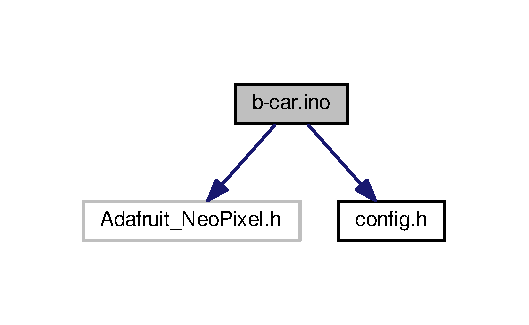
\includegraphics[width=254pt]{b-car_8ino__incl}
\end{center}
\end{figure}
\subsection*{Functions}
\begin{DoxyCompactItemize}
\item 
void \hyperlink{group__car_gaa0a39b0689218537e29a29f9c3f2af47}{normalmode} ()
\begin{DoxyCompactList}\small\item\em Normal operation mode. \end{DoxyCompactList}\end{DoxyCompactItemize}
{\bf }\par
\begin{DoxyCompactItemize}
\item 
void \hyperlink{group__main_ga4fc01d736fe50cf5b977f755b675f11d}{setup} ()
\begin{DoxyCompactList}\small\item\em Inital setup. \end{DoxyCompactList}\item 
void \hyperlink{group__main_gafe461d27b9c48d5921c00d521181f12f}{loop} ()
\begin{DoxyCompactList}\small\item\em Main loop. \end{DoxyCompactList}\end{DoxyCompactItemize}



\subsection{Detailed Description}
Main file. 

\begin{DoxyAuthor}{Author}
copyrights 
\end{DoxyAuthor}

\hypertarget{buttons_8ino}{}\section{buttons.\+ino File Reference}
\label{buttons_8ino}\index{buttons.\+ino@{buttons.\+ino}}


Use two R-\/2R resistor ladder networks to connect up to 10 buttons on two analog inputs.  


\begin{DoxyCompactItemize}
\item 
uint16\+\_\+t \hyperlink{group__buttons_gac23a04180ca7609f571853499faae915}{lastbuttons} = 0
\begin{DoxyCompactList}\small\item\em Last read of button pressed. \end{DoxyCompactList}\item 
uint16\+\_\+t \hyperlink{group__buttons_gaca8bc953fb5340b58c9403b3bf8bbd8e}{stablebuttons} = 0
\begin{DoxyCompactList}\small\item\em Pressed Buttons after debounce. \end{DoxyCompactList}\item 
uint16\+\_\+t \hyperlink{group__buttons_gac52f8abe18e87b9ce8cdba2e27bbbf02}{buttonstore} = \hyperlink{group__buttons_ga77a6549a849f9a9472a367e4148289b7}{T\+O\+G\+G\+L\+E\+M\+A\+SK}
\begin{DoxyCompactList}\small\item\em Stores push buttons as simulated toggle buttons. \end{DoxyCompactList}\item 
uint16\+\_\+t \hyperlink{group__buttons_gafa19e52bd127439ef22ade9f91753386}{buttonstate} = 0
\begin{DoxyCompactList}\small\item\em Stores current button state with simulated toggle buttons included. \end{DoxyCompactList}\item 
uint16\+\_\+t \hyperlink{group__buttons_gacc4c256fa5e75c09f1b3a669d45485ec}{rising} = 0
\begin{DoxyCompactList}\small\item\em Stores simulated interrupts for rising edge. \end{DoxyCompactList}\item 
uint16\+\_\+t \hyperlink{group__buttons_ga1861b594f36400f6c17b1f65b2565816}{falling} = 0
\begin{DoxyCompactList}\small\item\em Stores simulated interrupts for falling edge. \end{DoxyCompactList}\item 
uint16\+\_\+t \hyperlink{group__buttons_ga541db091bf54e0a51180f3666e5a2ce2}{rfilter} = 0
\begin{DoxyCompactList}\small\item\em Filter for simulated interrupts for rising edge. \end{DoxyCompactList}\item 
uint16\+\_\+t \hyperlink{group__buttons_gaaa75cede053f94cf46d7420556af1505}{ffilter} = 0
\begin{DoxyCompactList}\small\item\em Filter for simulated interrupts for falling edge. \end{DoxyCompactList}\item 
unsigned long \hyperlink{group__buttons_ga94921f7ca95d518d3deabb1da432c2fb}{dtime} = 0
\begin{DoxyCompactList}\small\item\em Store the time of the last debounce to calculate delta time to next debounce. \end{DoxyCompactList}\item 
void \hyperlink{group__buttons_gaf32fa88edc93b34e25f058e331ea1134}{update\+Buttons} ()
\begin{DoxyCompactList}\small\item\em Read button state and calculate stable button state. \end{DoxyCompactList}\item 
bool \hyperlink{group__buttons_gad4a8f6035320735a6ed69364c0f29d63}{button\+State} (uint16\+\_\+t mask)
\begin{DoxyCompactList}\small\item\em Returns the state of a button as boolean. \end{DoxyCompactList}\item 
uint16\+\_\+t \hyperlink{group__buttons_ga5421761bb5d1c3470d3b17196a438c80}{readr2r} (int pin)
\begin{DoxyCompactList}\small\item\em Calculated the current button state as a 5 bit mask. \end{DoxyCompactList}\item 
uint16\+\_\+t \hyperlink{group__buttons_ga0ce7c5a698df341a0f3882378518f562}{debounce} (uint16\+\_\+t curbuttons)
\begin{DoxyCompactList}\small\item\em Debounce button presses of the R-\/2R resistor ladder network. \end{DoxyCompactList}\item 
void \hyperlink{group__buttons_ga66c6a02c014dc9acd3af0c816a70fad8}{updintr} (uint16\+\_\+t state)
\begin{DoxyCompactList}\small\item\em Update the simulated interrupts of the R-\/2R resistor ladder network. \end{DoxyCompactList}\item 
uint16\+\_\+t \hyperlink{group__buttons_ga9b1decfe9116af4b8853a02aebfa1d14}{get\+Rising} (uint16\+\_\+t mask)
\begin{DoxyCompactList}\small\item\em Get simulated rising edge interrupt(s) for simulated interrupt service routine. \end{DoxyCompactList}\item 
uint16\+\_\+t \hyperlink{group__buttons_ga2971d62e0d7420f71836fb86e0fce92f}{get\+Falling} (uint16\+\_\+t mask)
\begin{DoxyCompactList}\small\item\em Get simulated falling edge interrupt(s) for simulated interrupt service routine. \end{DoxyCompactList}\end{DoxyCompactItemize}


\subsection{Detailed Description}
Use two R-\/2R resistor ladder networks to connect up to 10 buttons on two analog inputs. 

\begin{DoxyAuthor}{Author}
copyrights
\end{DoxyAuthor}
\begin{DoxySeeAlso}{See also}
\href{https://en.wikipedia.org/wiki/Resistor_ladder#R.E2.80.932R_resistor_ladder_network_.28digital_to_analog_conversion.29}{\tt https\+://en.\+wikipedia.\+org/wiki/\+Resistor\+\_\+ladder\#\+R.\+E2.\+80.\+932\+R\+\_\+resistor\+\_\+ladder\+\_\+network\+\_\+.\+28digital\+\_\+to\+\_\+analog\+\_\+conversion.\+29} 
\end{DoxySeeAlso}

\hypertarget{car__basics_8ino}{}\section{car\+\_\+basics.\+ino File Reference}
\label{car__basics_8ino}\index{car\+\_\+basics.\+ino@{car\+\_\+basics.\+ino}}


Basic car functionality.  


\subsection*{Functions}
{\bf }\par
\begin{DoxyCompactItemize}
\item 
void \hyperlink{group__car_gaca3b725ebee32d3719a9c02b41002ea3}{turn\+\_\+right} ()
\begin{DoxyCompactList}\small\item\em Activate right turn lights. \end{DoxyCompactList}\item 
void \hyperlink{group__car_ga0565ad7a822d9d334bb50c088af22361}{turn\+\_\+left} ()
\begin{DoxyCompactList}\small\item\em Activate left turn lights. \end{DoxyCompactList}\item 
void \hyperlink{group__car_ga6b1fd674445dd1c654dfe8b8b65f168e}{beam} (unsigned long state)
\begin{DoxyCompactList}\small\item\em Activate low beam or high beam. \end{DoxyCompactList}\item 
void \hyperlink{group__car_ga29d5eff542aae0196b8e84b8a752e1df}{low\+\_\+beam} (bool on)
\item 
void \hyperlink{group__car_ga1088d06b4ab015d579e0ac2510d39f25}{high\+\_\+beam} (bool on)
\item 
void \hyperlink{group__car_gac7295d1018b2b948084ba5dbacf09d74}{tacho} ()
\begin{DoxyCompactList}\small\item\em Display the current speed on tacho\+\_\+row L\+E\+Ds. \end{DoxyCompactList}\item 
void \hyperlink{group__car_gaffb7c011f82f3fb47b39ebb2713a1cd8}{flash} ()
\begin{DoxyCompactList}\small\item\em Flash light. \end{DoxyCompactList}\end{DoxyCompactItemize}



\subsection{Detailed Description}
Basic car functionality. 

\begin{DoxyAuthor}{Author}
copyrights 
\end{DoxyAuthor}
\begin{DoxyRefDesc}{Todo}
\item[\hyperlink{todo__todo000001}{Todo}]Write a function for brake lights. \end{DoxyRefDesc}

\hypertarget{config_8h}{}\section{config.\+h File Reference}
\label{config_8h}\index{config.\+h@{config.\+h}}


Adjust your settings here.  


This graph shows which files directly or indirectly include this file\+:\nopagebreak
\begin{figure}[H]
\begin{center}
\leavevmode
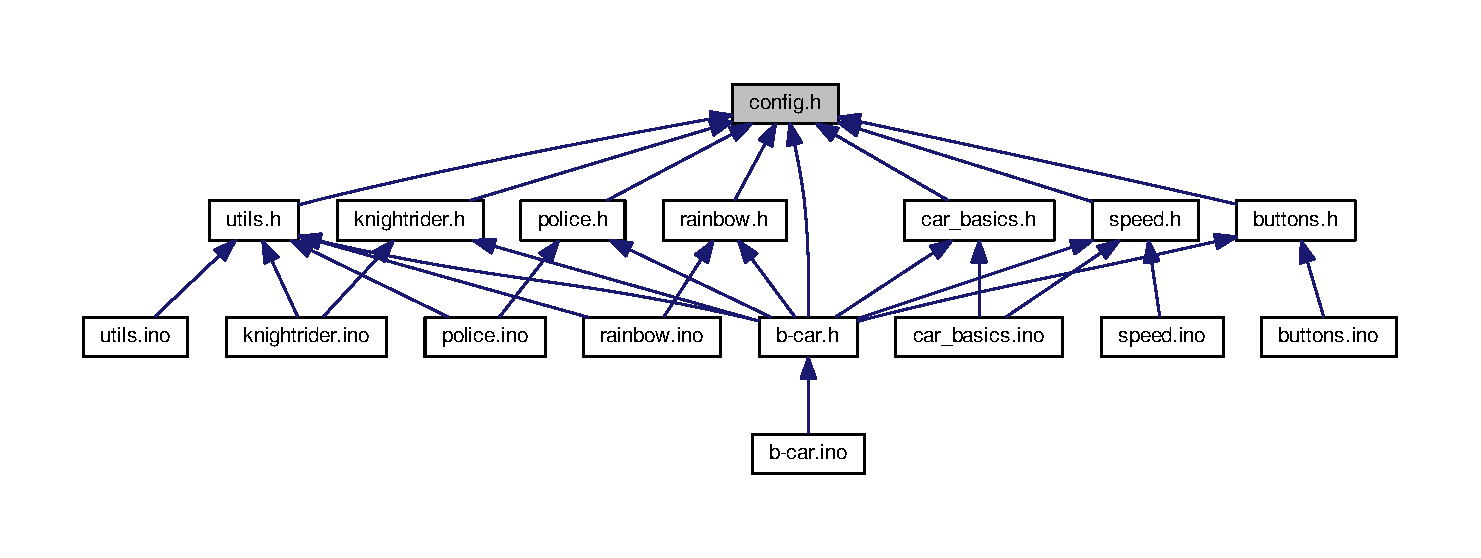
\includegraphics[width=134pt]{config_8h__dep__incl}
\end{center}
\end{figure}
\subsection*{Macros}
\begin{DoxyCompactItemize}
\item 
\#define \hyperlink{group__buttons_gab47d09cf51ee6fbdc1b7b255f57ec896}{B\+U\+T\+T\+O\+N\+S1}~A1
\begin{DoxyCompactList}\small\item\em Define analog input for first five buttons. \end{DoxyCompactList}\item 
\#define \hyperlink{group__buttons_gac3f0a90f8f8169f919f346be1ea485db}{B\+U\+T\+T\+O\+N\+S2}~A2
\begin{DoxyCompactList}\small\item\em Define analog input for second five buttons. \end{DoxyCompactList}\item 
\#define \hyperlink{group__buttons_ga171ef18ea7b584f85234640a918da857}{D\+E\+B\+O\+U\+N\+CE}~20
\begin{DoxyCompactList}\small\item\em Define delay in ms to debounce button presses. \end{DoxyCompactList}\item 
\#define \hyperlink{group__buttons_ga0dae655e00097db2f5737cef9f1fe1e6}{S5}~0b0000000001
\begin{DoxyCompactList}\small\item\em Bit mask for button 5. \end{DoxyCompactList}\item 
\#define \hyperlink{group__buttons_gac6dd50ea82e237280daf26bd9b562ba9}{S4}~0b0000000010
\begin{DoxyCompactList}\small\item\em Bit mask for button 4. \end{DoxyCompactList}\item 
\#define \hyperlink{group__buttons_gab29872af8ce9dc9463b7f7ecfbea02ae}{S3}~0b0000000100
\begin{DoxyCompactList}\small\item\em Bit mask for button 3. \end{DoxyCompactList}\item 
\#define \hyperlink{group__buttons_gad5e70dee3c36d645b0eb1743b8a7d2bf}{S2}~0b0000001000
\begin{DoxyCompactList}\small\item\em Bit mask for button 2. \end{DoxyCompactList}\item 
\#define \hyperlink{group__buttons_ga690d30e9ad3647835c243368b36d4c41}{S1}~0b0000010000
\begin{DoxyCompactList}\small\item\em Bit mask for button 1. \end{DoxyCompactList}\item 
\#define \hyperlink{group__buttons_ga1ff88b4fe56e1c80a371b1fbda4e4e74}{S10}~0b0000100000
\begin{DoxyCompactList}\small\item\em Bit mask for button 10. \end{DoxyCompactList}\item 
\#define \hyperlink{group__buttons_ga6eef6bdffd8bac54d6b4be0176dd20ff}{S9}~0b0001000000
\begin{DoxyCompactList}\small\item\em Bit mask for button 9. \end{DoxyCompactList}\item 
\#define \hyperlink{group__buttons_ga4516955061f24ae7162de20aff005c9b}{S8}~0b0010000000
\begin{DoxyCompactList}\small\item\em Bit mask for button 8. \end{DoxyCompactList}\item 
\#define \hyperlink{group__buttons_ga6580eeddd36d0d97cdde6f6a4695ed12}{S7}~0b0100000000
\begin{DoxyCompactList}\small\item\em Bit mask for button 7. \end{DoxyCompactList}\item 
\#define \hyperlink{group__buttons_gab86bfbee3d71830e88c61a3f8d5aebf4}{S6}~0b1000000000
\begin{DoxyCompactList}\small\item\em Bit mask for button 6. \end{DoxyCompactList}\item 
\#define \hyperlink{group__buttons_ga77a6549a849f9a9472a367e4148289b7}{T\+O\+G\+G\+L\+E\+M\+A\+SK}~0b1110000000
\begin{DoxyCompactList}\small\item\em Bit mask for simulated toggle buttons. \end{DoxyCompactList}\item 
\#define \hyperlink{group__car_ga6670c8646da7675376960bb5773199fd}{T\+U\+R\+N\+L\+I\+G\+HT}~0xffc000
\begin{DoxyCompactList}\small\item\em Color of turn lights. \end{DoxyCompactList}\item 
\#define \hyperlink{group__car_ga61bb8d5dab460079c1b621b2d8a4bd9c}{L\+O\+W\+B\+E\+AM}~0x3f3f3f
\begin{DoxyCompactList}\small\item\em Color of low beam. \end{DoxyCompactList}\item 
\#define \hyperlink{group__car_ga3f561f12573270e4b5329bc5930ad20f}{H\+I\+G\+H\+B\+E\+AM}~0x7f7f7f
\begin{DoxyCompactList}\small\item\em Color of high beam. \end{DoxyCompactList}\item 
\#define \hyperlink{group__car_gae97ccf06dd29b2a0500f378068b678e2}{B\+A\+C\+K\+L\+I\+G\+HT}~0x3f0000
\begin{DoxyCompactList}\small\item\em Color of back lights. \end{DoxyCompactList}\item 
\#define \hyperlink{group__knightrider_ga5d96b8b7a94cd393a11cca853832350f}{K\+RR}~0x7f
\begin{DoxyCompactList}\small\item\em Red part of Knight Rider like front row. \end{DoxyCompactList}\item 
\#define \hyperlink{group__knightrider_ga47a5cb8daecea854270c0d09c3ebc24c}{K\+RG}~0x00
\begin{DoxyCompactList}\small\item\em Green part of Knight Rider like front row. \end{DoxyCompactList}\item 
\#define \hyperlink{group__knightrider_gaa315fefb5665924b7d512104bc3965cd}{K\+RB}~0x00
\begin{DoxyCompactList}\small\item\em Blue part of Knight Rider like front row. \end{DoxyCompactList}\item 
\#define \hyperlink{group__knightrider_gadb436e031abc2aed3e3cbbf9078667bb}{K\+R\+P\+E\+R\+I\+OD}~500
\begin{DoxyCompactList}\small\item\em Period in ms the Knight Rider like front row needs to move in one direction. \end{DoxyCompactList}\item 
\#define \hyperlink{group__knightrider_ga64a0c208656bb11ad944489886089b7e}{K\+R\+D\+TZ}~200
\begin{DoxyCompactList}\small\item\em Fade out period in ms for a smooth light flow. \end{DoxyCompactList}\item 
\#define \hyperlink{group__police_ga088f4c3612d1ab1c9f6f139234ae533b}{PR}~0x00
\begin{DoxyCompactList}\small\item\em Red part of the police beacon light. \end{DoxyCompactList}\item 
\#define \hyperlink{group__police_ga037f1be1c3e45bf4d0d4f5ddc159ff30}{PG}~0x00
\begin{DoxyCompactList}\small\item\em Green part of the police beacon light. \end{DoxyCompactList}\item 
\#define \hyperlink{group__police_ga2a06f3773d46878dc58f8dadd6fd0d72}{PB}~0xff
\begin{DoxyCompactList}\small\item\em Blue part of the police beacon light. \end{DoxyCompactList}\item 
\#define \hyperlink{group__police_gaa5b3f73b18472f543c080194bf9c2e79}{P\+P\+E\+R\+I\+OD}~1000
\begin{DoxyCompactList}\small\item\em Rotation period in ms of the police beacon light. \end{DoxyCompactList}\item 
\#define \hyperlink{group__police_ga2b9a2b71c1aa4f1c059461e2db7edf44}{P\+D\+TZ}~200
\begin{DoxyCompactList}\small\item\em Fade out period in ms for a smooth light flow. \end{DoxyCompactList}\item 
\#define \hyperlink{group__police_ga6204e236d3e4ef0beb5b6fd976fecf43}{P\+L\+F\+L\+A\+SH}~0xff0000
\begin{DoxyCompactList}\small\item\em Left side flash color of the police front row. \end{DoxyCompactList}\item 
\#define \hyperlink{group__police_ga98673c164f8917ff7af0016ba30e7ca8}{P\+L\+L\+OW}~0x1f0000
\begin{DoxyCompactList}\small\item\em Left side low light color of the police front row. \end{DoxyCompactList}\item 
\#define \hyperlink{group__police_gac9d0142b6f8cc7735af13e6b91503b97}{P\+R\+F\+L\+A\+SH}~0x0000ff
\begin{DoxyCompactList}\small\item\em Right side flash color of the police front row. \end{DoxyCompactList}\item 
\#define \hyperlink{group__police_gaf4a707e896c2e6df7a0215e4100d75aa}{P\+R\+L\+OW}~0x00001f
\begin{DoxyCompactList}\small\item\em Right side low light color of the police front row. \end{DoxyCompactList}\item 
\#define \hyperlink{group__rainbow_ga36ae3bd3da884ff03d7306f674f70dea}{R\+B\+S\+T\+EP}~40
\begin{DoxyCompactList}\small\item\em Rainbow step size between two L\+E\+Ds. \end{DoxyCompactList}\item 
\#define \hyperlink{group__speed_ga984097794e94beb18c01b6fcbd8f399d}{I\+N\+T\+E\+R\+R\+U\+P\+T\+P\+IN}~P\+C\+I\+N\+T1
\begin{DoxyCompactList}\small\item\em This is P\+B1 per the schematic. \end{DoxyCompactList}\item 
\#define \hyperlink{group__speed_ga77b45027297b1ff40b5b1249afb852e5}{P\+C\+I\+N\+T\+\_\+\+V\+E\+C\+T\+OR}~P\+C\+I\+N\+T0\+\_\+vect
\item 
\#define \hyperlink{group__speed_ga9142f4c677315955ad0ac6266b615d2c}{D\+A\+T\+A\+D\+I\+R\+E\+C\+T\+I\+O\+N\+P\+IN}~D\+D\+B1
\item 
\#define \hyperlink{group__speed_gaab113cddfa5f8856918dcb65238882ca}{P\+O\+R\+T\+P\+IN}~P\+B1
\item 
\#define \hyperlink{group__speed_ga93a1139e66a97ca289f0f1a73903be06}{R\+E\+A\+D\+P\+IN}~P\+I\+N\+B1
\item 
\#define \hyperlink{group__deployment_gae1a27401b7fb01ccb9a82dbddbb54eea}{P\+IN}~0
\item 
\#define \hyperlink{group__deployment_ga4c4ae9a4146ce8d6a5debc90300d9abd}{N\+U\+M\+\_\+\+L\+E\+DS}~32
\end{DoxyCompactItemize}
\subsection*{Variables}
\begin{DoxyCompactItemize}
\item 
const byte \hyperlink{group__deployment_gac03fd0ab9cbcc53730039ad03e9b094d}{turn\+\_\+light\+\_\+left} \mbox{[}$\,$\mbox{]} =\{17,27\}
\item 
const byte \hyperlink{group__deployment_ga1a25903a2850d9849775664473070489}{low\+\_\+beam\+\_\+row} \mbox{[}$\,$\mbox{]} =\{1,2,16,15\}
\item 
const byte \hyperlink{group__deployment_ga1ecea646e1c5dcdfc643287a5f2041bb}{high\+\_\+beam\+\_\+row} \mbox{[}$\,$\mbox{]} = \{1,2,16,15\}
\item 
const byte \hyperlink{group__deployment_ga5009aa0cbe6b32a72b085489b027800e}{front\+\_\+row} \mbox{[}$\,$\mbox{]} = \{3,4,5,13,14\}
\item 
const byte \hyperlink{group__deployment_ga6ade605406f4c1ce9f03a5a2530f6dbe}{tacho\+\_\+row} \mbox{[}$\,$\mbox{]} = \{12,11,10,9,8,7,6\}
\item 
const byte \hyperlink{group__deployment_gaa5a6ee27fdf1d7c939cdf2a7266d7e84}{turn\+\_\+light\+\_\+right} \mbox{[}$\,$\mbox{]} =\{0,30\}
\item 
const byte \hyperlink{group__deployment_gaac36c9836edd3a125668213f0fb72b5a}{down\+\_\+left\+\_\+row} \mbox{[}$\,$\mbox{]} = \{18,19,20,21\}
\item 
const byte \hyperlink{group__deployment_gadbf10ff9ee353128c568e07c32b1ffa9}{down\+\_\+right\+\_\+row} \mbox{[}$\,$\mbox{]} = \{22,23,24,25\}
\item 
const byte \hyperlink{group__deployment_ga516415cfaebc59b71f822fb4cf86b22c}{back\+\_\+light\+\_\+row} \mbox{[}$\,$\mbox{]} = \{26,28,29,31\}
\item 
const byte \hyperlink{group__deployment_gad4e8497757364dbc8187298bd87acc44}{rainbowrow\+\_\+left} \mbox{[}$\,$\mbox{]} = \{5,13,14,17,15,16,18,19,20,21,30,31,29, 9,10,11,12\}
\item 
const byte \hyperlink{group__deployment_ga00c047fede9a8b6c020ba1d108d63cea}{rainbowrow\+\_\+right} \mbox{[}$\,$\mbox{]} = \{5, 4, 3, 0, 2, 1,22,23,24,25,27,26,28, 9, 8, 7, 6\}
\item 
Adafruit\+\_\+\+Neo\+Pixel \hyperlink{group__deployment_gacf2771bd8bfaf855bbcc6c30301bf380}{strip} = Adafruit\+\_\+\+Neo\+Pixel(\hyperlink{group__deployment_ga4c4ae9a4146ce8d6a5debc90300d9abd}{N\+U\+M\+\_\+\+L\+E\+DS}, \hyperlink{group__deployment_gae1a27401b7fb01ccb9a82dbddbb54eea}{P\+IN}, N\+E\+O\+\_\+\+R\+GB + N\+E\+O\+\_\+\+K\+H\+Z800)
\item 
static volatile unsigned long \hyperlink{group__main_ga4f944bfefd58754546ebcc7c5143442c}{time}
\begin{DoxyCompactList}\small\item\em Global accessable variable that stores the current time after program start in ms. \end{DoxyCompactList}\item 
byte \hyperlink{group__main_ga988166baebc4b27bd18de27cd40f8b5a}{mode} =0
\begin{DoxyCompactList}\small\item\em stores current operation mode \end{DoxyCompactList}\end{DoxyCompactItemize}


\subsection{Detailed Description}
Adjust your settings here. 

\begin{DoxyAuthor}{Author}
copyrights 
\end{DoxyAuthor}

\hypertarget{knightrider_8ino}{}\section{knightrider.\+ino File Reference}
\label{knightrider_8ino}\index{knightrider.\+ino@{knightrider.\+ino}}


Knight Rider like front row.  


{\ttfamily \#include \char`\"{}knightrider.\+h\char`\"{}}\\*
{\ttfamily \#include \char`\"{}utils.\+h\char`\"{}}\\*
Include dependency graph for knightrider.\+ino\+:\nopagebreak
\begin{figure}[H]
\begin{center}
\leavevmode
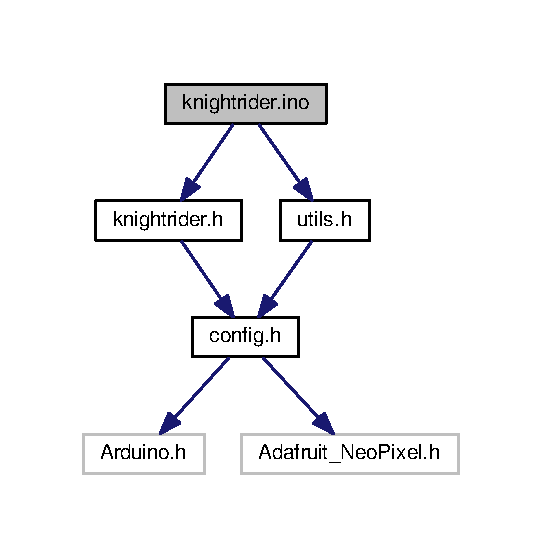
\includegraphics[width=260pt]{knightrider_8ino__incl}
\end{center}
\end{figure}
\subsection*{Functions}
{\bf }\par
\begin{DoxyCompactItemize}
\item 
void \hyperlink{group__knightrider_ga58bfb7b9f8fcf7a4b02700359057a6f4}{knightrider} ()
\begin{DoxyCompactList}\small\item\em Knight Rider like front row. \end{DoxyCompactList}\end{DoxyCompactItemize}



\subsection{Detailed Description}
Knight Rider like front row. 

\begin{DoxyAuthor}{Author}
copyrights 
\end{DoxyAuthor}

\hypertarget{police_8ino}{}\section{police.\+ino File Reference}
\label{police_8ino}\index{police.\+ino@{police.\+ino}}


Police beacon light and front flash.  


\subsection*{Functions}
{\bf }\par
\begin{DoxyCompactItemize}
\item 
void \hyperlink{group__police_ga55d627c45708bc26866e27d49432eee9}{police} ()
\item 
void \hyperlink{group__police_ga82542db5e1a84d584a1725f36caaf71e}{p\+\_\+front} (boolean ls, boolean rs, boolean left)
\end{DoxyCompactItemize}



\subsection{Detailed Description}
Police beacon light and front flash. 

\begin{DoxyAuthor}{Author}
copyrights 
\end{DoxyAuthor}
\begin{DoxyRefDesc}{Todo}
\item[\hyperlink{todo__todo000003}{Todo}]May add more flasher. 

Extract beacon light as seperate function. \end{DoxyRefDesc}

\hypertarget{rainbow_8ino}{}\section{rainbow.\+ino File Reference}
\label{rainbow_8ino}\index{rainbow.\+ino@{rainbow.\+ino}}


Rainbow effect functions.  


\subsection*{Functions}
{\bf }\par
\begin{DoxyCompactItemize}
\item 
void \hyperlink{group__rainbow_ga51e30a1c423190e50127c6651c991612}{rainbowmode} ()
\item 
void \hyperlink{group__rainbow_ga3656f41cfe48a0bf63e63099673ac4c4}{underbody\+\_\+rb} ()
\item 
void \hyperlink{group__rainbow_ga80198b192c269a2b71cfa41654a3aafd}{rainbow} (byte led, byte pos, byte distance)
\end{DoxyCompactItemize}



\subsection{Detailed Description}
Rainbow effect functions. 

\begin{DoxyAuthor}{Author}
copyrights 
\end{DoxyAuthor}
\begin{DoxyRefDesc}{Todo}
\item[\hyperlink{todo__todo000004}{Todo}]Make period of rainbow cycle configurable in \hyperlink{config_8h}{config.\+h} \end{DoxyRefDesc}

\hypertarget{speed_8ino}{}\section{speed.\+ino File Reference}
\label{speed_8ino}\index{speed.\+ino@{speed.\+ino}}


Measure speed.  


{\ttfamily \#include \char`\"{}speed.\+h\char`\"{}}\\*
Include dependency graph for speed.\+ino\+:\nopagebreak
\begin{figure}[H]
\begin{center}
\leavevmode
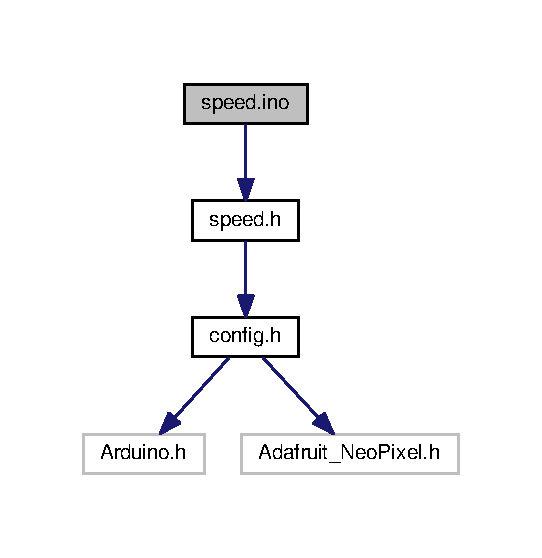
\includegraphics[width=260pt]{speed_8ino__incl}
\end{center}
\end{figure}
\begin{DoxyCompactItemize}
\item 
unsigned long \hyperlink{group__speed_ga605bafc427aaa8e9718a112441ba88a7}{speedts}
\item 
unsigned long \hyperlink{group__speed_ga66ce79a1ea6b700d56211c146f679649}{braketime}
\item 
unsigned int \hyperlink{group__speed_ga63232e097931bc02aa65b3b7dadbb74b}{curspeed}
\item 
bool \hyperlink{group__speed_gad13fd9ed7295daa9a51dd2fade080e50}{isbraking}
\item 
void \hyperlink{group__speed_gae87a94769934715c309733cfdf2abcb4}{setup\+\_\+interrupt} ()
\item 
\hyperlink{group__speed_ga44395845abd4a9c31e4fbe88ed717fa3}{I\+SR} (\hyperlink{group__speed_ga77b45027297b1ff40b5b1249afb852e5}{P\+C\+I\+N\+T\+\_\+\+V\+E\+C\+T\+OR})
\item 
unsigned int \hyperlink{group__speed_gafc7b1718f9b23966dfed24056f67996f}{getspeed} ()
\begin{DoxyCompactList}\small\item\em Get current speed. \end{DoxyCompactList}\item 
void \hyperlink{group__speed_gaa41dbc9d264f533090ac3c808c43171f}{acceleration} (unsigned int newspeed)
\begin{DoxyCompactList}\small\item\em Test for negative accelaration (braking) \end{DoxyCompactList}\item 
bool \hyperlink{group__speed_ga3ad56507af5eec4c270def2058efbc3b}{braking} ()
\begin{DoxyCompactList}\small\item\em Braking information. \end{DoxyCompactList}\item 
void \hyperlink{group__speed_ga2004678343c1f7b145dc10aae949a4ec}{resetspeed} ()
\item 
byte \hyperlink{group__speed_gaa1b4f1cc5cf5ba94e3bc38f44e0c7001}{getspeedidx} ()
\end{DoxyCompactItemize}


\subsection{Detailed Description}
Measure speed. 

\begin{DoxyAuthor}{Author}
copyrights 
\end{DoxyAuthor}
\begin{DoxyRefDesc}{Todo}
\item[\hyperlink{todo__todo000005}{Todo}]Write a function that detects braking via negative acceleration. \end{DoxyRefDesc}

\hypertarget{utils_8ino}{}\section{utils.\+ino File Reference}
\label{utils_8ino}\index{utils.\+ino@{utils.\+ino}}


Collection of utils.  


{\ttfamily \#include \char`\"{}utils.\+h\char`\"{}}\\*
Include dependency graph for utils.\+ino\+:\nopagebreak
\begin{figure}[H]
\begin{center}
\leavevmode
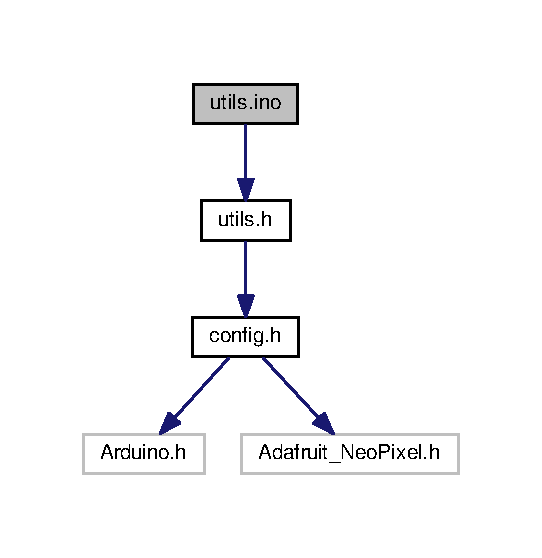
\includegraphics[width=260pt]{utils_8ino__incl}
\end{center}
\end{figure}
\subsection*{Functions}
\begin{DoxyCompactItemize}
\item 
void \hyperlink{utils_8ino_a798729dca95209ecdc609807a653a2bf}{clear\+All} ()
\item 
uint8\+\_\+t \hyperlink{utils_8ino_ab5a87ca857f392dbad3bf3a4582c3f0e}{fade8} (uint16\+\_\+t distance, uint16\+\_\+t dtz)
\item 
uint8\+\_\+t \hyperlink{utils_8ino_ae7f706e9934c4154b7a4e222f14c8c9a}{percent8} (uint8\+\_\+t full, uint8\+\_\+t fac)
\item 
uint8\+\_\+t \hyperlink{group___fast_l_e_d_ga538b510f61cc75c8e4491f9f2797ee7c}{sin8} (uint8\+\_\+t theta)
\item 
uint8\+\_\+t \hyperlink{group___fast_l_e_d_ga007b62e82ea1556ea7b0e3d2656bce09}{cos8} (uint8\+\_\+t theta)
\item 
uint32\+\_\+t \hyperlink{group___adafruit_ga953424274959481c9d46b57d249b3722}{Wheel} (byte Wheel\+Pos)
\begin{DoxyCompactList}\small\item\em Input a value 0 to 255 to get a color value. The colours are a transition r -\/ g -\/ b -\/ back to r. \end{DoxyCompactList}\end{DoxyCompactItemize}


\subsection{Detailed Description}
Collection of utils. 

\begin{DoxyAuthor}{Author}
copyrights 
\end{DoxyAuthor}


\subsection{Function Documentation}
\index{utils.\+ino@{utils.\+ino}!clear\+All@{clear\+All}}
\index{clear\+All@{clear\+All}!utils.\+ino@{utils.\+ino}}
\subsubsection[{\texorpdfstring{clear\+All()}{clearAll()}}]{\setlength{\rightskip}{0pt plus 5cm}void clear\+All (
\begin{DoxyParamCaption}
{}
\end{DoxyParamCaption}
)}\hypertarget{utils_8ino_a798729dca95209ecdc609807a653a2bf}{}\label{utils_8ino_a798729dca95209ecdc609807a653a2bf}


Definition at line 8 of file utils.\+ino.

\index{utils.\+ino@{utils.\+ino}!fade8@{fade8}}
\index{fade8@{fade8}!utils.\+ino@{utils.\+ino}}
\subsubsection[{\texorpdfstring{fade8(uint16\+\_\+t distance, uint16\+\_\+t dtz)}{fade8(uint16_t distance, uint16_t dtz)}}]{\setlength{\rightskip}{0pt plus 5cm}uint8\+\_\+t fade8 (
\begin{DoxyParamCaption}
\item[{uint16\+\_\+t}]{distance, }
\item[{uint16\+\_\+t}]{dtz}
\end{DoxyParamCaption}
)}\hypertarget{utils_8ino_ab5a87ca857f392dbad3bf3a4582c3f0e}{}\label{utils_8ino_ab5a87ca857f392dbad3bf3a4582c3f0e}


Definition at line 14 of file utils.\+ino.

\index{utils.\+ino@{utils.\+ino}!percent8@{percent8}}
\index{percent8@{percent8}!utils.\+ino@{utils.\+ino}}
\subsubsection[{\texorpdfstring{percent8(uint8\+\_\+t full, uint8\+\_\+t fac)}{percent8(uint8_t full, uint8_t fac)}}]{\setlength{\rightskip}{0pt plus 5cm}uint8\+\_\+t percent8 (
\begin{DoxyParamCaption}
\item[{uint8\+\_\+t}]{full, }
\item[{uint8\+\_\+t}]{fac}
\end{DoxyParamCaption}
)}\hypertarget{utils_8ino_ae7f706e9934c4154b7a4e222f14c8c9a}{}\label{utils_8ino_ae7f706e9934c4154b7a4e222f14c8c9a}


Definition at line 23 of file utils.\+ino.


%--- End generated contents ---

% Index
\backmatter
\newpage
\phantomsection
\clearemptydoublepage
\addcontentsline{toc}{chapter}{Index}
\printindex

\end{document}
